
{\chapter{Single  cell  whole genome fitness  landscapes  induced  by pharmacologic perturbations in cancer}
}
\label{ch:Chapter4}

\section{Motivation}
As discussed in introduction chapter 1, tumor fitness landscape underpin selection in cancer evolution and response to chemotherapy. However,quantifying fitness in heterogeneous tumor populations remains an open problem that hampers effective treatment leading to tumor recurrence. Previous work has established models of fitness through interpreting allelic measurements of single snapshots \cite{Williams2016-of,Williams2018-ga,Gerstung2020-jl,shah2012clonal,Nik-Zainal2012-uk} from bulk sequencing over large patient cohorts \cite{martincorena2017universal}, timeseries study of cell free DNA \cite{Khan2018-uj}, multiregion sequencing \cite{Gerlinger2014-qd,Jamal-Hanjani2017-yc,Lopez2020-ku,mcpherson2016divergent,williams2018quantification} and estimating fitness landscapes of clonal haematopoiesis \cite{Watson2020-yu}. Moreover, the cancer field has generally lacked serial measurements from patient derived tissues to directly observe cancer evolution over realistic timescales. This has impeded a thorough understanding of causal factors driving selection, achieved in other biological systems through studying granular timeseries with population genetics modeling \cite{Good2017-fv}. The majority of the work on cancer has focused on bulk tumour sequencing, where cellular population structure decomposition approaches are limited. Single cell genome measurements to scalably define clonal populations in cancer over thousands of cells have only recently emerged \cite{Laks2019-dm,zahn2017scalable}, enabling identification of rare populations, precise tracking of clones and robust clone-specific measurements suitable for population genetics modeling. We are also motivated by newly developed quantifying 
tools of sitka, a phylogenetic inference method accompanying toolkits to assign cells to clones, \cite{dorri2020efficient} and 
\texttt{fitClone}, a probabilistic framework that designates quantitative selection coefficients to individual cancer clones and forecasts competitive clonal dynamics over time \cite{salehi2020single}.

\section{Synopsis}
Based on the knowledge we gained from chapter 3, three \ac{PDX} tumors and two drugs were selected to investigate clonal dynamics and identify patterns of clonal resistance with single cell whole genome sequencing. First, we generated two serially transplanted timeseries PDX (SA535-HER2+ and SA609-TNBC) from passage one (X1) to passage ten (X10) to test the newly developed methods (from collaborators) for identifying sub-populations with their genotypes.
We showed that serial measurements of single cell copy number assigned clones can be used to estimate fitness in conjunction with \texttt{fitClone} \cite{salehi2020single}, under serial transplantation of breast patient derived xenografts, where no drug selection or other conditions were applied. We found that serial measurements can be used to measure relative clonal fitness which enables prediction of future trajectories.

Next we sought to  confirm the reproducibility and independence of dynamics to population size effects, we re-ran the serial transplantation experiments after mixing early and late populations and re-measuring the dynamical behaviour. We observed that sufficiently well sampled clones with confident fitness estimations show repeated trajectories, confirming the estimation of fitness and linking the dynamical behaviour to the copy number genotypes of the clones.

Finally, we determined whether the fitness of clones under chemotherapy can be measured and asked whether clones exhibiting drug resistance are also fitter in the absence of selective pressure from chemotherapy. 

On all the single cell whole genome sequencing data, we applied three types of scientific computational methodologies. First, \textbf{sitka},  for computing phylogenetic trees and identifying genotypic clones, then using \textbf{Lumberjack} (a tree-cutting algorithm) and their relative abundances as a function of time. Last, \texttt{fitClone}, to measure the selection coefficient for each clone \textit{s} which we hypothesise to indicate growth potential. The larger the value of \textit{s}, the more fit the clone is relative to the chosen reference clone. 

%...........................................................





\section{Results}

 
\subsection{Establishment of untreated timeseries patient derived xenografts}
Taking multiple measurements is critical for understanding  given behavior of cancer clones that are forced to evolve over time, and doing so at equal intervals give an open opportunity to clearly investigate the dynamics of that behavior manifesting at distinct time scales. 
To understand and quantify fitness attributes of cancer cells as  predictive measures of their growth potential in polyclonal systems, we set out to establish time series patient derived xenografts (PDX) with and without pharmacological perturbations.
Serial transplantations were performed by injecting patient derived tumor cells and clumps into primary engrafted mice to secondary and subsequent recipients in a time series manner \textbf{(Figure 4.1, n=3-4 at each time point)}. We passaged two PDX, SA532 (HER2+) and SA609 (TNBC), till tenth generation (X1-X10). X1 represents passage one (first generation) of the PDX and X10 as last passage (tenth generation) \textbf{(Figure 4.1 a)}. Tumor growth measurements record from both PDX serries exhibited increased growth rate in later passages as compared to early passages \textbf{(Figure 4.1 b)}.
 
 
 \begin{figure}
\centering
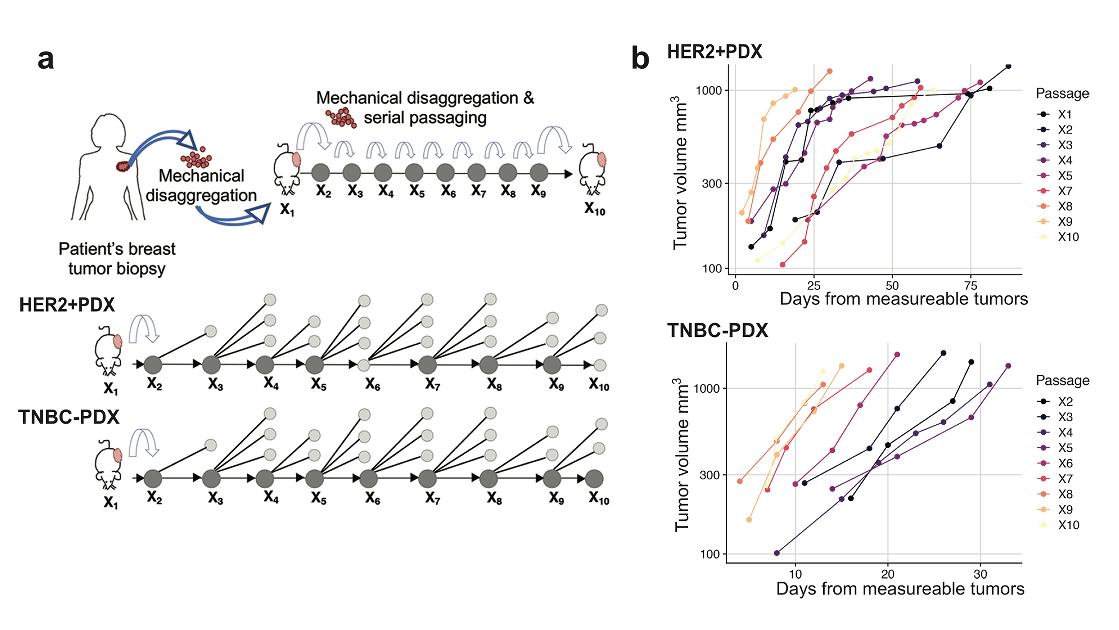
\includegraphics[width=\textwidth]{Figures/Untreatedgrowthcurves.pdf}
	
\caption[Untreated PDX timeseries and growth trajectories]
	{\small
	\textbf{Untreated PDX timeseries and growth trajectories.}
	    \textbf{(a)}, Top: Schematic for PDX timeseries; Bottom: Serial sampling of HER2+ and TNBC PDX tumours;
Dark grey circles represent each sampled mouse for scWGS. The light grey circles representing the replicates of tumour-bearing mice at the same timepoint. Small light grey at X6 and X10 represents absent data points.
	    \textbf{(b)}, Individual tumour growth from each passage of TNBC and HER2+ PDXs. Y-axis is showing the tumor volume in cubic millimeter while the x-axis is representing the time in days, tumors could be measured.
	}
	\label{fig:Untreated timeseries growth curves only}
\end{figure}

\begin{figure}
\centering
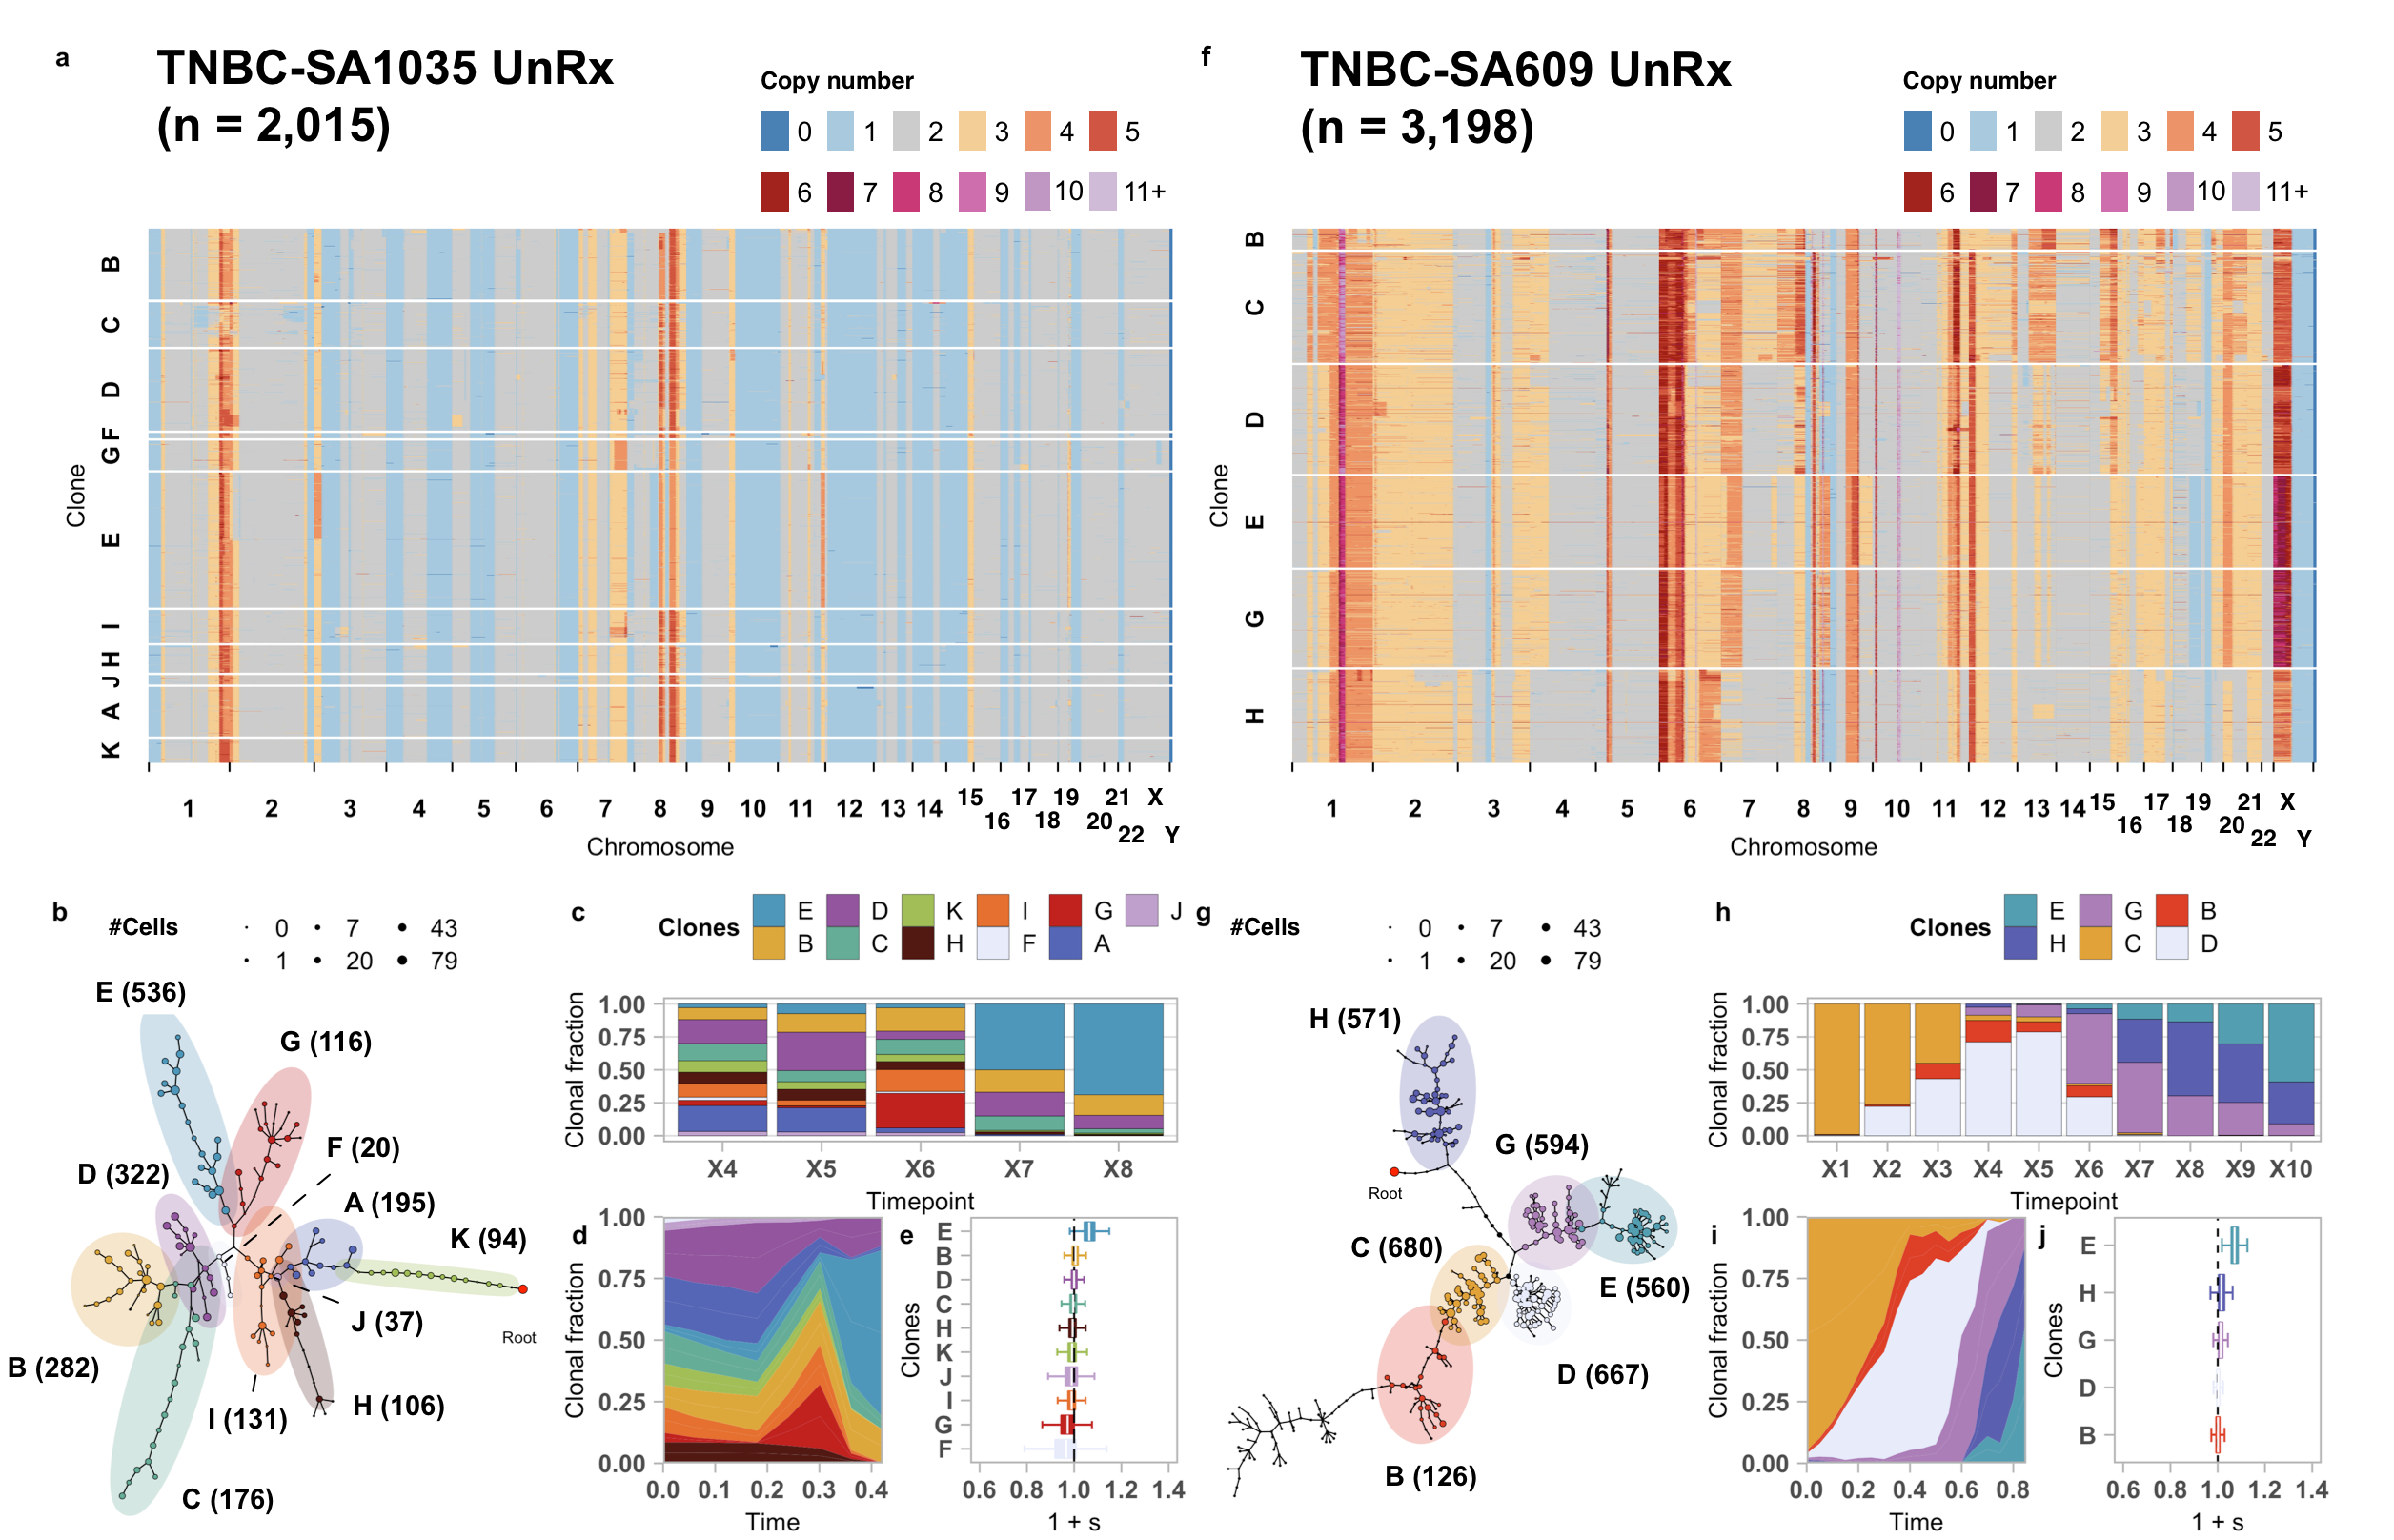
\includegraphics[width=\textwidth]{Figures/UnRxseries.pdf}
	
\caption[Untreated PDX timeseries clonal dynamics at single cell level]
	{\small
	\textbf{Comparison of fitness landscapes of two untreated breast cancer PDX timeseries models.}
	    \textbf{(a, b)} Clonal dynamics of HER2+ and TNBC models.
	    \textbf{(c)} Probability of positive selection in both PDx
	    \textbf{(d)} Heatmap representation of copy number profiles of 2,193 cells, grouped in 4 phylogenetic clades. 
	    \textbf{(e)} Phylogeny (simplified type II sitka tree) of cells over the timeseries HER2+ Untreated PDX, where nodes are groups of cells (scaled in size by number) with shared copy number genotype and edges represent distinct genomic copy number change points (sitka markers)
 
\textbf{(f)} Top: growth trajectories, Bottom: Inferred \texttt{fitClone} trajectories
\textbf{(g)} selection coefficients for the HER2+ model. 
 \textbf{(h-k)} Analogous plots for the TNBC model (n=3,216 cells).
 
	}
	\label{fig:Untreated timeseries growth curves only}
\end{figure}


 Patient's tumor architecture and integrity was confirmed on H \& E and immuno-histochemistry staining of paraffin embedded tumor sections at each time point with a set of standard markers. \textbf{(See Methods, Figure 2.1 a, b)} showing representative images of initial and late passages of tumor sections.

\subsection{Clone-specific fitness estimates forecast clonal competition trajectories} 
 
 We next generated single cell whole genomes from 10 serial PDX transplants over 721 days from a HER2+ breast cancer with a \textit{TP53} p.A159P missense mutation, and contrasted this with 10 serial samples over 1002 days from a basal-like \ac{TNBC} PDX with a \textit{TP53} p.R213* non-sense mutation. Two time points, X6 and X10 from HER2 positive PDX failed to produce successful library so those were removed during analysis. Clonal expansions observed during serial passaging of \textit{TP53} mutant PDX tumours to determine the predictive capacity of fitness coefficients \textbf{Figure 4.3}.
A median of 907 single cell genomes were sequenced per passage for a total of 11,705 and 10,553 single cell genomes from the HER2+ and TNBC series, respectively. 


\subsubsection{Phylogenetics and fitness analysis on single cell whole genome data}
For each of the two timeseries PDX, we inferred single cell copy number profiles, constructed a phylogenetic tree using \textbf{sitka} model taking copy number states as input to establish clonal lineages and measured clonal abundances as a function of time. For each timeseries (branch), we pulled all single cells to infer a phylogenetic tree \textbf{(See introduction and methods for details)}. The tree was cut using Lumberjack to yield clones and their abundances over time. Then \texttt{fitClone} inferred selection coefficient of a clone by reporting the posterior mean 1 + s followed by its standard deviation.

\subsubsection{Untreated timeseries SA532 HER2+ PDX undergo neutral clonal dynamics}
 The SA532 HER2+ series exhibited 4 distinct clones ranging in size from 134 to 1,421 cells (median 319, \textbf{Figure 4.2 e)}, and the TNBC series exhibited 8 distinct clones with 18 to 680 cells (median 556, \textbf{Figure 4.2 i)}. Clonal trajectories in the HER2+ model, were consistent with selective coefficients with small relative differences in fitness \textbf{(Figure 4.2 f, g)}.
 We observed a small decrease of 0.04 copy number breakpoints per generation (linear regression, p=0.002,=0.05). 

\subsubsection{Untreated timeseries SA609 TNBC PDX undergo deterministic clonal dynamics}
In contrast to HER2+ timeseries, the TNBC model trajectories resulted in a high positive selective coefficient for a minority of clones \textbf{(Figure 4.2 j, k)} mean = 1.03 $\pm $0.11. Consistent with increased dynamics in the TNBC series, we found an initial increase of 0.1 breakpoints per cell per generation in the first 4 passages  \textbf{(Figure A.1 a)}). After this initial increase the average number of breakpoints per cell remained constant.
 Clone E in TNBC swept the population over the last 3 timepoints \textbf{(Figure 4.2 j, k)} (n=541 over the timeseries). Clone E had the highest selective coefficient (1+s= 1.08 $\pm $ 0.043), having grown from undetectable proportions in earlier timepoints to 58\% of cells by the end of the timeseries. Clone E also had the highest number of breakpoints with 12.8 additional copy number breakpoints per cell, relative to the reference clone C with the lowest (linear regression with coverage breadth, ploidy and cell cycle state as covariates (p $<$0.0001) \textbf{(Figure A.1 c)}.


\subsection{SA609-TNBC mixture timeseries yielded selection of biologically similar population}
We next asked whether the high predicted fitness of Clone E was a true indicator of positive selection through a physical clonal mixing and re-transplant experiment. Enforced clonal competition of higher fitness clones with lower fitness counterparts should result in re-emergence or fixation of high fitness clones, even when re-starting from a low population prevalence. To test this, we performed mixture experiments by extracting cells from an early (X3) and a late (X8) passage of SA609 TNBC timeseries PDX
and then physically mix them. We established two such lines with different prorportions \textbf{(also see methods)}
In first branch a, we aimed to have a mixture comprising approximately of equal proportions from the two
timepoints ($\approx$~50\% each) at the ratio of 1:1. In branch b, we aimed to have far less cells from late passage that contains the high fitness clone. The (71\% of X3 passage and 29.0\% of cells from the X8 passage) a ratio of 1:0.4.


\subsubsection{Clones with higher selection coefficients out compete low fitness clones in mixture branch a}
We forward-simulated trajectories from \texttt{fitClone} using the median of the posterior distribution of the estimated selection coefficients (F = -0.01  $\pm$ 0.13, A = -0.00 $\pm$ 0.16, B= 0.00 $\pm$  0.01, D = 0.00  $\pm$  0.01, G = 0.02  $\pm$  0.02, H = 0.03  $\pm$  0.03, E = 0.08  $\pm$ 0.10) and starting clonal proportions of (A=0.000 (no observed cells), B=0.07, C=0.25, D=0.51, E=0.02, F=0.000 (no observed cells), G=0.08 H=0.07) \textbf{Figure 4.3 a,f}. The starting clonal proportions were inferred by adding the cells from the initial passage (M0) to the tree inferred from the cells in the original series (TNBC-SA609) and assigning them to their respective clones. We generated 10,000 trajectories from the model. \textbf{Figure 4.3 c} shows the simulated trajectories in black.
The mean clonal fraction at each step is shown in red. All clones except for clones E, D, and F are predicted to vanish to clonal fractions of below 1\%. We have combined the trajectories for clones E and F since clone F (i) had fewer than 19 total cells in the original series and consequently its selection coefficient had a high variance, (ii) is phylogenetically proximal to clone E \textbf{Figure 4.3 b} and thus likely represented a biologically similar population and (iii) finally, is not observed above a threshold of 20 cells in any other line in the TNBC-SA609 family.

We experimentally tested these predictions by initiating a new PDX line with the remixed population (from M0), serially passaged over 4 timepoints \textbf{Figure 4.3 a} (top), and sequenced with DLP+ (7,839 single cell genomes, median 1,354.5 per library). After placing the cells from all timepoints of this mixture experiment on the tree, they got assigned to seven clones from the original timeseries (all but clone A) between 26 to 499 (median 162) cells \textbf{Figure 4.3 d} . In \textbf{Figure 4.3 c, f} blue dots show the observed clonal fractions at each timepoint in PDX branch a. Clones with higher selection co-efficients swept through the mixture timeseries by passage 4 \textbf{Figure 4.3 e}. In the last timepoint, the clade composed of clones E and F comprised 94\% of cells, outcompeting low-fitness clones. The estimated selection co-efficients were relatively strongly correlated (Pearson correlation of 0.795, considering only clones that reached overall prevalence of over 1\% in the original series, i.e., all clones except A and F.



\begin{figure}
\centering
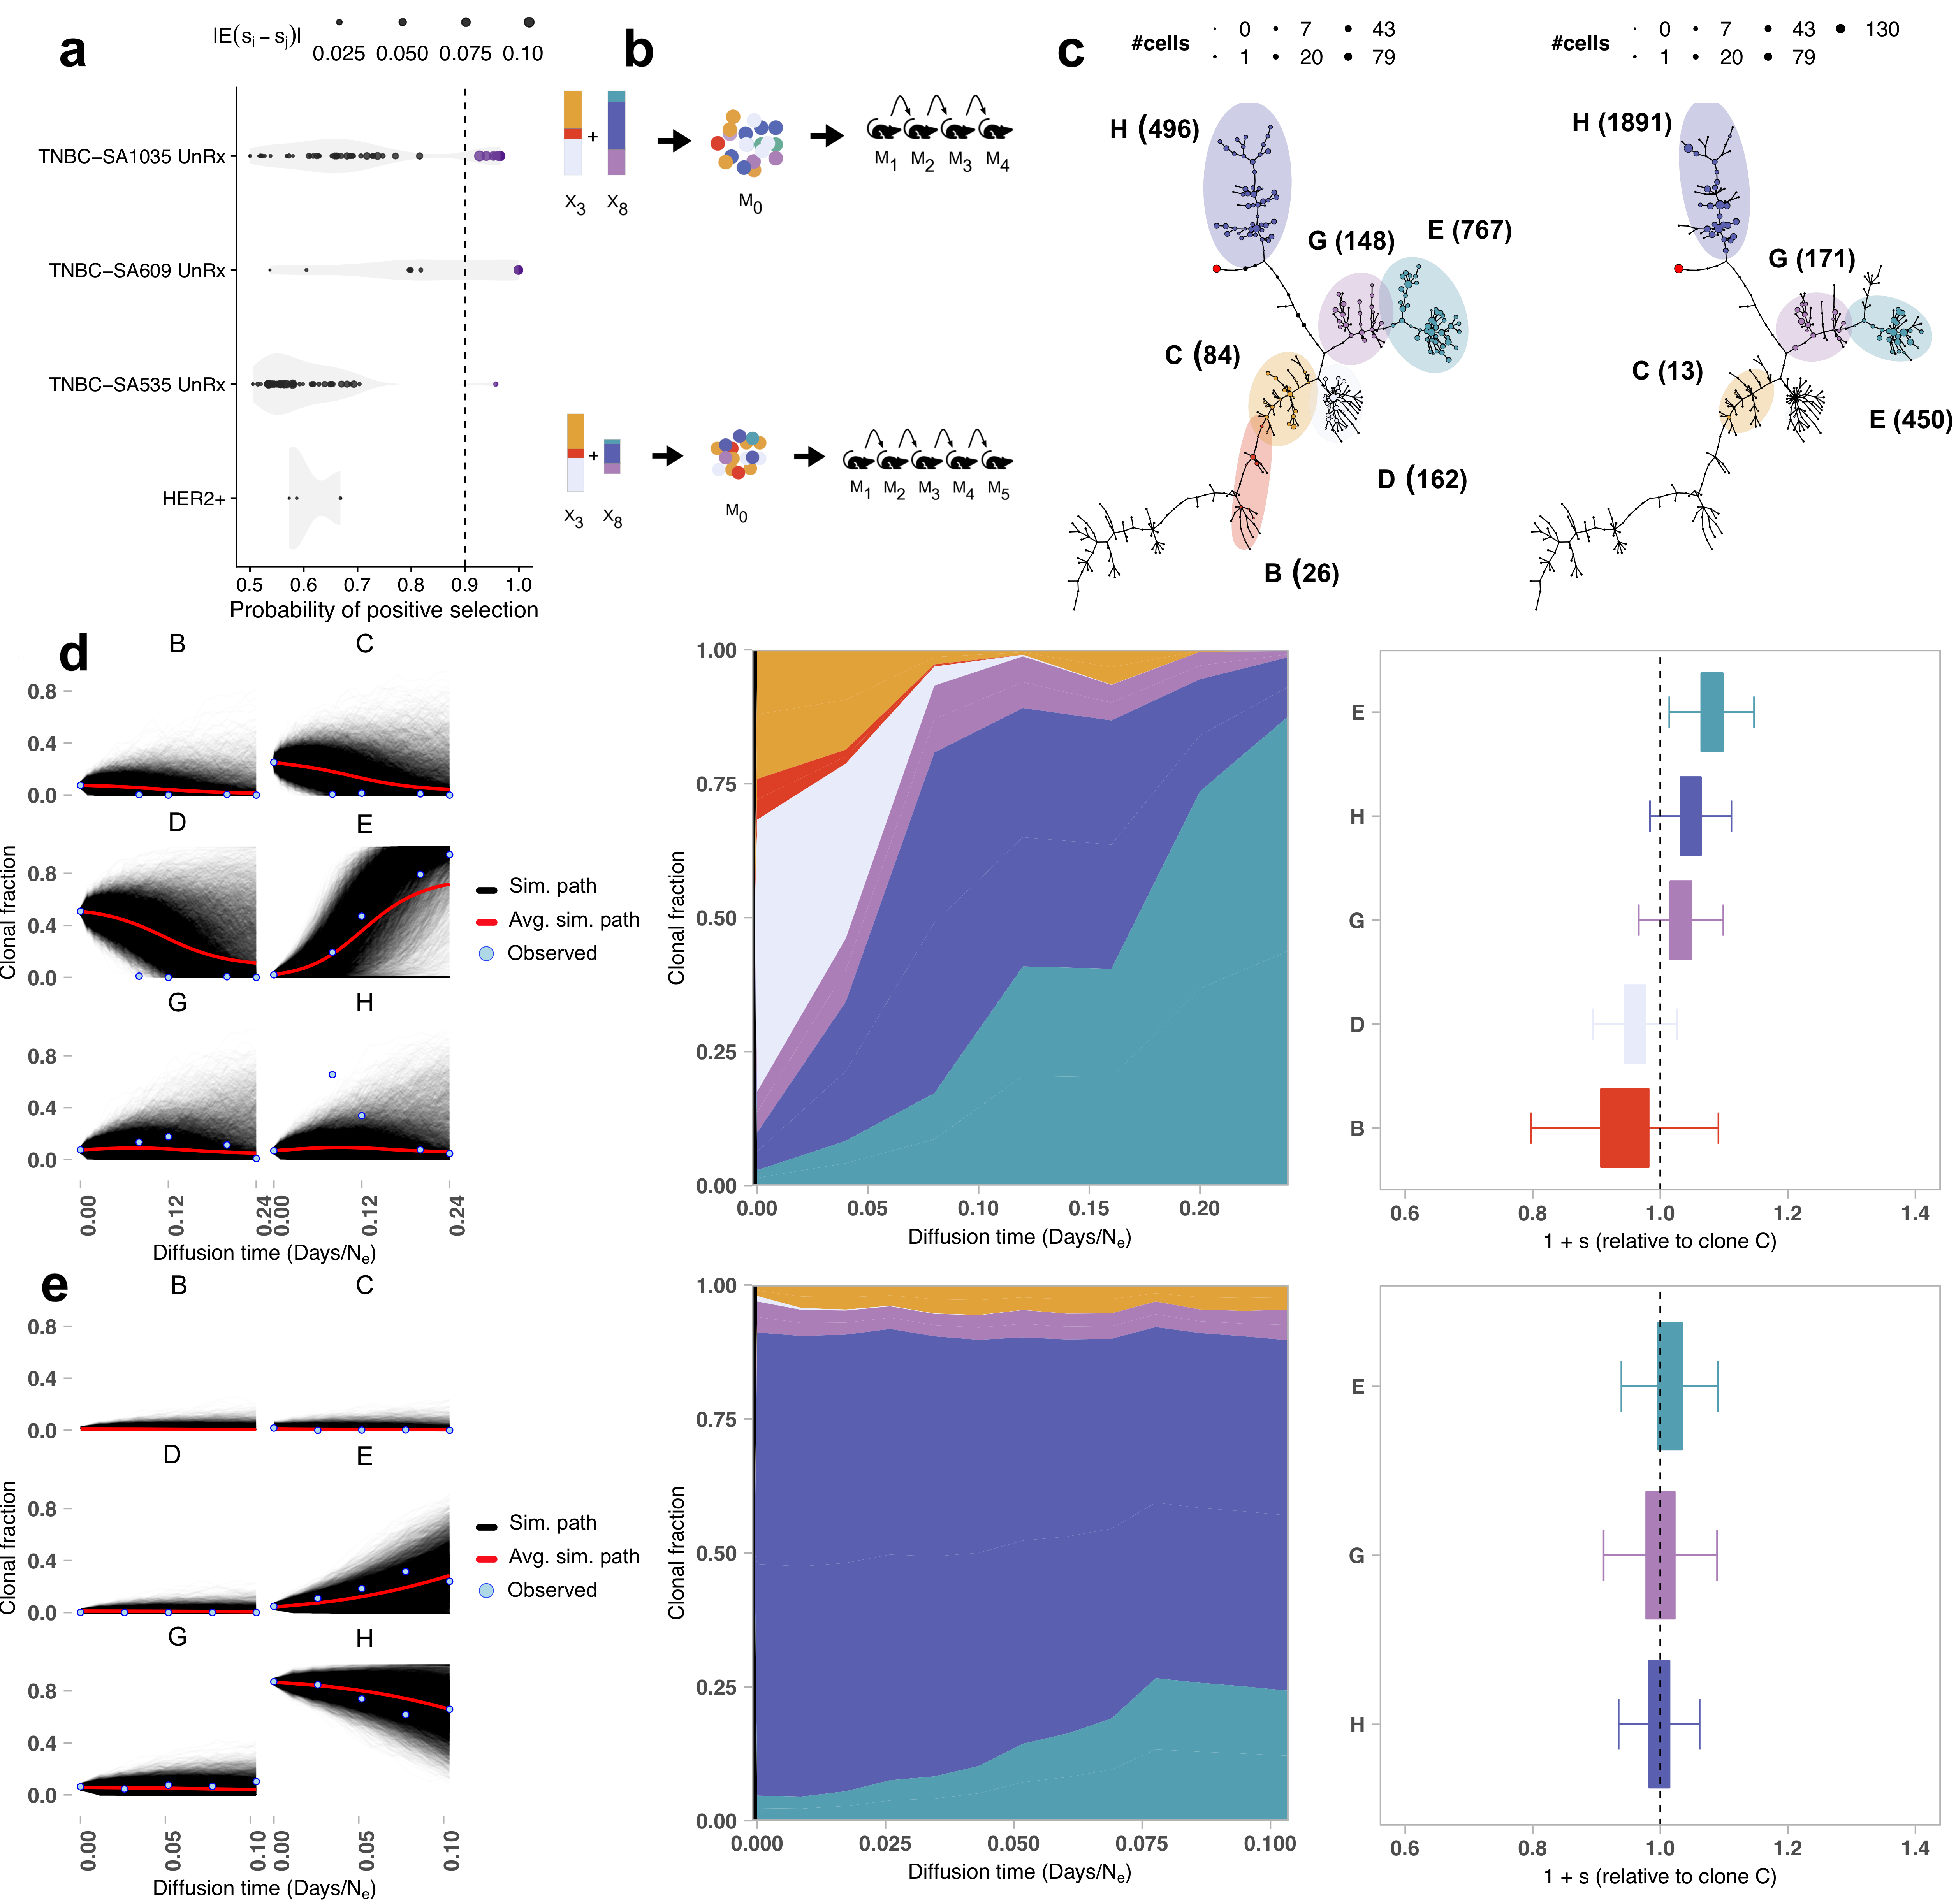
\includegraphics[width=\textwidth]{Figures/Mixturenew.pdf}
	
\caption[Reproducible dynamics from SA609-TNBC mixture experiments]
	{\small
	\textbf{Reproducible dynamics from SA609-TNBC mixture experiments}
	    \textbf{(a)} Clonal proportions of X3 and X8 to generate the initial mixture M0 and subsequent serial passaging, yielding 4 samples M1-M4 for mixture a and 5 samples
M1-M5 for mixture b.
	    \textbf{(b)} Phylogenies showing cells observed in the mixture a (left) and mixture b (right) timeseries.
	     \textbf{(c)} For mixture a: Forward simulations using inferred selection coefficients and starting population proportions in the initial experimental mixture. Red line representing the time-axis for the observations that is shrunk to best match the mean predicted trajectories
	     \textbf{(d)} Inferred trajectories of mixture a timeseries \textbf{(e)} Selection coefficients of \texttt{fitClone} fit to M1-M4 clonal abundance observations.
 \textbf{(f)} For mixture b: Forward simulations using inferred selection coefficients and starting population proportions in the initial experimental mixture
  \textbf{(g)} Inferred trajectories of mixture b timeseries
	  \textbf{(h)} Selection coefficients of \texttt{fitClone} fit to
M1-M5 clonal abundance observations.    
}
	\label{fig:Untreated timeseries growth curves only}
\end{figure}



\subsubsection{Mixture branch b recapitulates the predicted dynamics of branch a and the original untreated branch}
We forward simulated 10,000 trajectories using identical selection coefficient values as the first mixture branch a, but different clonal proportions, estimated from adding cells from timepoint X1 in mixture branch b to the TNBC-SA609 phylogenetic tree and assigning them to the corresponding clones (C = 0.02, D = 0.00, E = 0.05, F = 0.00, G = 0.06, H = 0.87). Unlike mixture branch a, DLP+ data was not available for timepoint M0 in mixture branch b. We generated a timeseries PDX passaged over 5 timepoints that were sequenced using the DLP+ platform to generate 6,730 single cell genomes (median 1,270 per library). We observed 6 clones from the original series, namely all clones except A and B. However, we only captured over the 5 timepoints, 1 cell from clone D, 8 cells from clone F, and 13 cells from clone C. As predicted, clone E, which had the highest predicted selection coefficient in the original series despite having started from a very low clonal fraction (0.05), rises to an abundance of 0.28, while clone H steadily falls from 0.87 to about 0.67 \textbf{(Figure 4.3 g, h)}.

The analysis of the two mixture series suggests that (i) we can validate the selection coefficients estimated from a timeseries using \texttt{fitClone} and (ii) it is possible make quantitative predictions about the likely trajectories of tumour subpopulations at least at the clade level. Also,in the prediction trajectories plot \textbf{Figure 4.3 c, f}, the time-axis for the observations is shrunk to best match the mean predicted trajectories line (red line). The diffusion time horizon that is obtained by dividing the generation time measured in days by the effective population size estimate results in trajectories that are ahead of the biological system. While in branch a the original time horizon is 0.24 and the best matching time is 0.20, in branch b the values are 0.23 and 0.08 respectively.





\begin{figure}
\centering
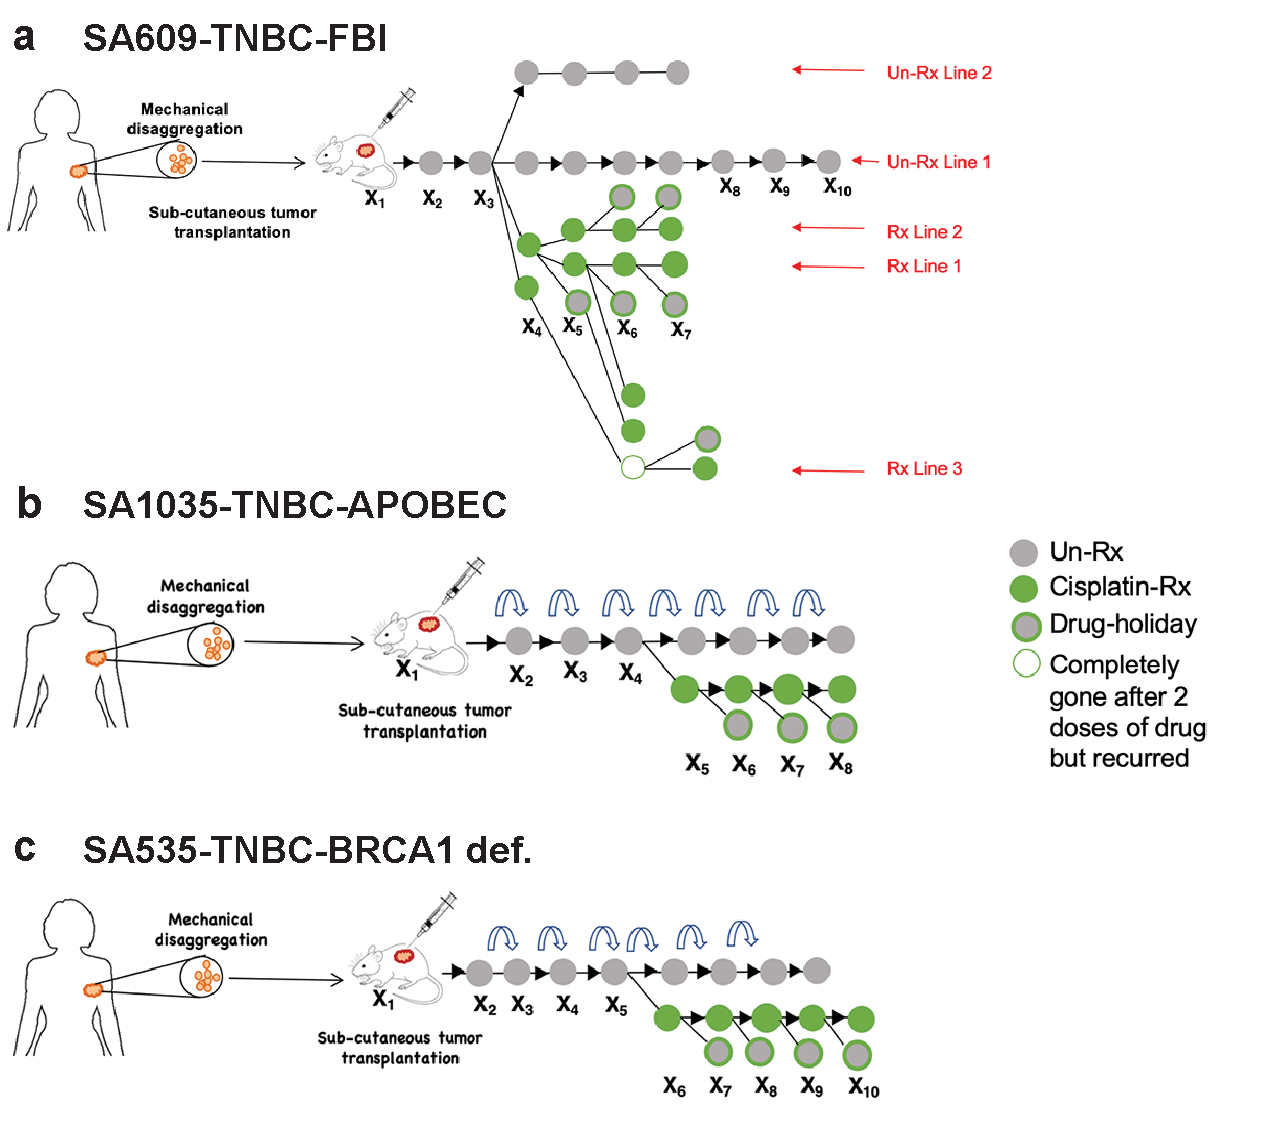
\includegraphics[width=\textwidth]{Figures/treatedtimeseriesgreen.pdf}
	
\caption[Experimental overview of TNBC PDX treated time series]
	{\small
	\textbf{Experimental overview of TNBC PDX treated time series.}
	      All nodes representing each PDX tumour were digested to acquire genomes of single cells (~200-600 cells/tumor). Extra replicate tumors at each time point are not shown in the diagram (n=2-4). Grey circles represent un-treated, green represents Cisplatin treated and grey with green outline presents drug-holiday samples \textbf{(a)} SA609-TNBC time series with replicate treated and un-treated branches. DLP+ collected starting from X1 to X10 (Un-Rx line 1). Top grey branch indicating Un-Rx line 2. The middle three branches are cisplatin treated time series replicate branches \textbf{(b)} SA535-TNBC  showing the tumor nodes taken for DLP+ starting from X5 untreated \textbf{(c)} SA1035-TNBC  showing the tumor nodes taken for DLP+ starting from X 4 untreated.}
	
	\label{fig:Untreated timeseries growth curves only}
\end{figure}

%...............................................................
\subsection{Clonal competition and fitness costs of platinum resistance}
So far we have applied our framework to pharmacologically unperturbed tumor environment to track human cancer clones as identified by their Copy number genotypes over time and to reason about their likely abundances and validating them with various experimental conditions. Now we investigate whether establishing baseline fitness measures could help to interpret selection under drug administration. We first present the TNBC-SA609 series in detail and make an observation about early response to cisplatin treatment. We then analyse two
additional TNBC PDX lines to check the reproduabiblty and generalizability of our observation.

\subsubsection{Repeated platinum exposure causes less tumor responsiveness} 
 To test pharmacologic perturbation with cisplatin (platinum) impacted the stability of the fitness landscape of the TNBC series, we generated a separate branch of the SA609-TNBC PDX model where we administered cisplatin (2mg/kg, \textit{Q3Dx8} i.p. max) serially over four successive passages to induce drug resistance along with its un treated control branch. For each serially treated tumour, a parallel set of transplanted mice were left untreated, establishing corresponding drug ‘holiday’ samples (\textbf{(See methods for detailed experimental design 1.1.4, Figure 2.2 a)}. Briefly, We coded the treated passages with 'T' and untreated with 'U' initialised by the X3 untreated (U) passage in SA609 TNBC, X4 untreated (U) in SA1035 TNBC and X5 untreated (U) in SA535 TNBC \textbf{Figure 4.4 a, b, c}. In SA609 TNBC, the first treatment passage(\textit{X4 UT}) exhibited rapid tumour shrinkage (>50\% of initial size). However \textit{X5 UTT}, \textit{X6 UTTT} and \textit{X7 UTTTT} had progressively less response, indicating drug resistance and positive growth kinetics \textbf{Figure 4.5}. 


\subsubsection{A new clone evolved and swept to fixation with increasing platinum cycles in SA609-TNBC PDX}
Decomposing the growth dynamics over (\textit{X3 U}; \textit{X4 UT}; \textit{X5 UTT}; \textit{X6 UTTT}; \textit{X7 UTTTT}) into clonal trajectories with DLP+ analysis suggested sustained cisplatin treatment inverted the fitness landscape. A new Clone R,  derived from Clone A in the phylogeny, but with a distinct clonal genotype (fewer copies of \textit{MYC} and deletions at \textit{RB1}, \textit{PRDM9} and \textit{NUDT15} loci \textbf{Figure 4.6 a, b}, swept to fixation comprising 48\% (\textit{X4 UT}), 98\% (\textit{X5 UTT}), 100\% (\textit{X6 UTTT}) and 100\% (\textit{X7 UTTTT}) of cells across the treated series \textbf{Figure 4.6 c}. Notably, the high fitness clones E, H, G, D from the untreated series exhibited low fitness coefficients in the treatment series and were no longer detected \textbf{Figure 4.6 d, 4.11}. Conversely, Clones A, and B, comprising a low fitness phylogenetic superclade, distinct from high fitness clones E and F in the untreated series, were the precursors to the resistant clone R \textbf{Figure 4.7 d, 4.11}. Thus, cisplatin perturbation resulted in a near complete inversion of the fitness landscape.

%....................................................................


\begin{figure}
\centering
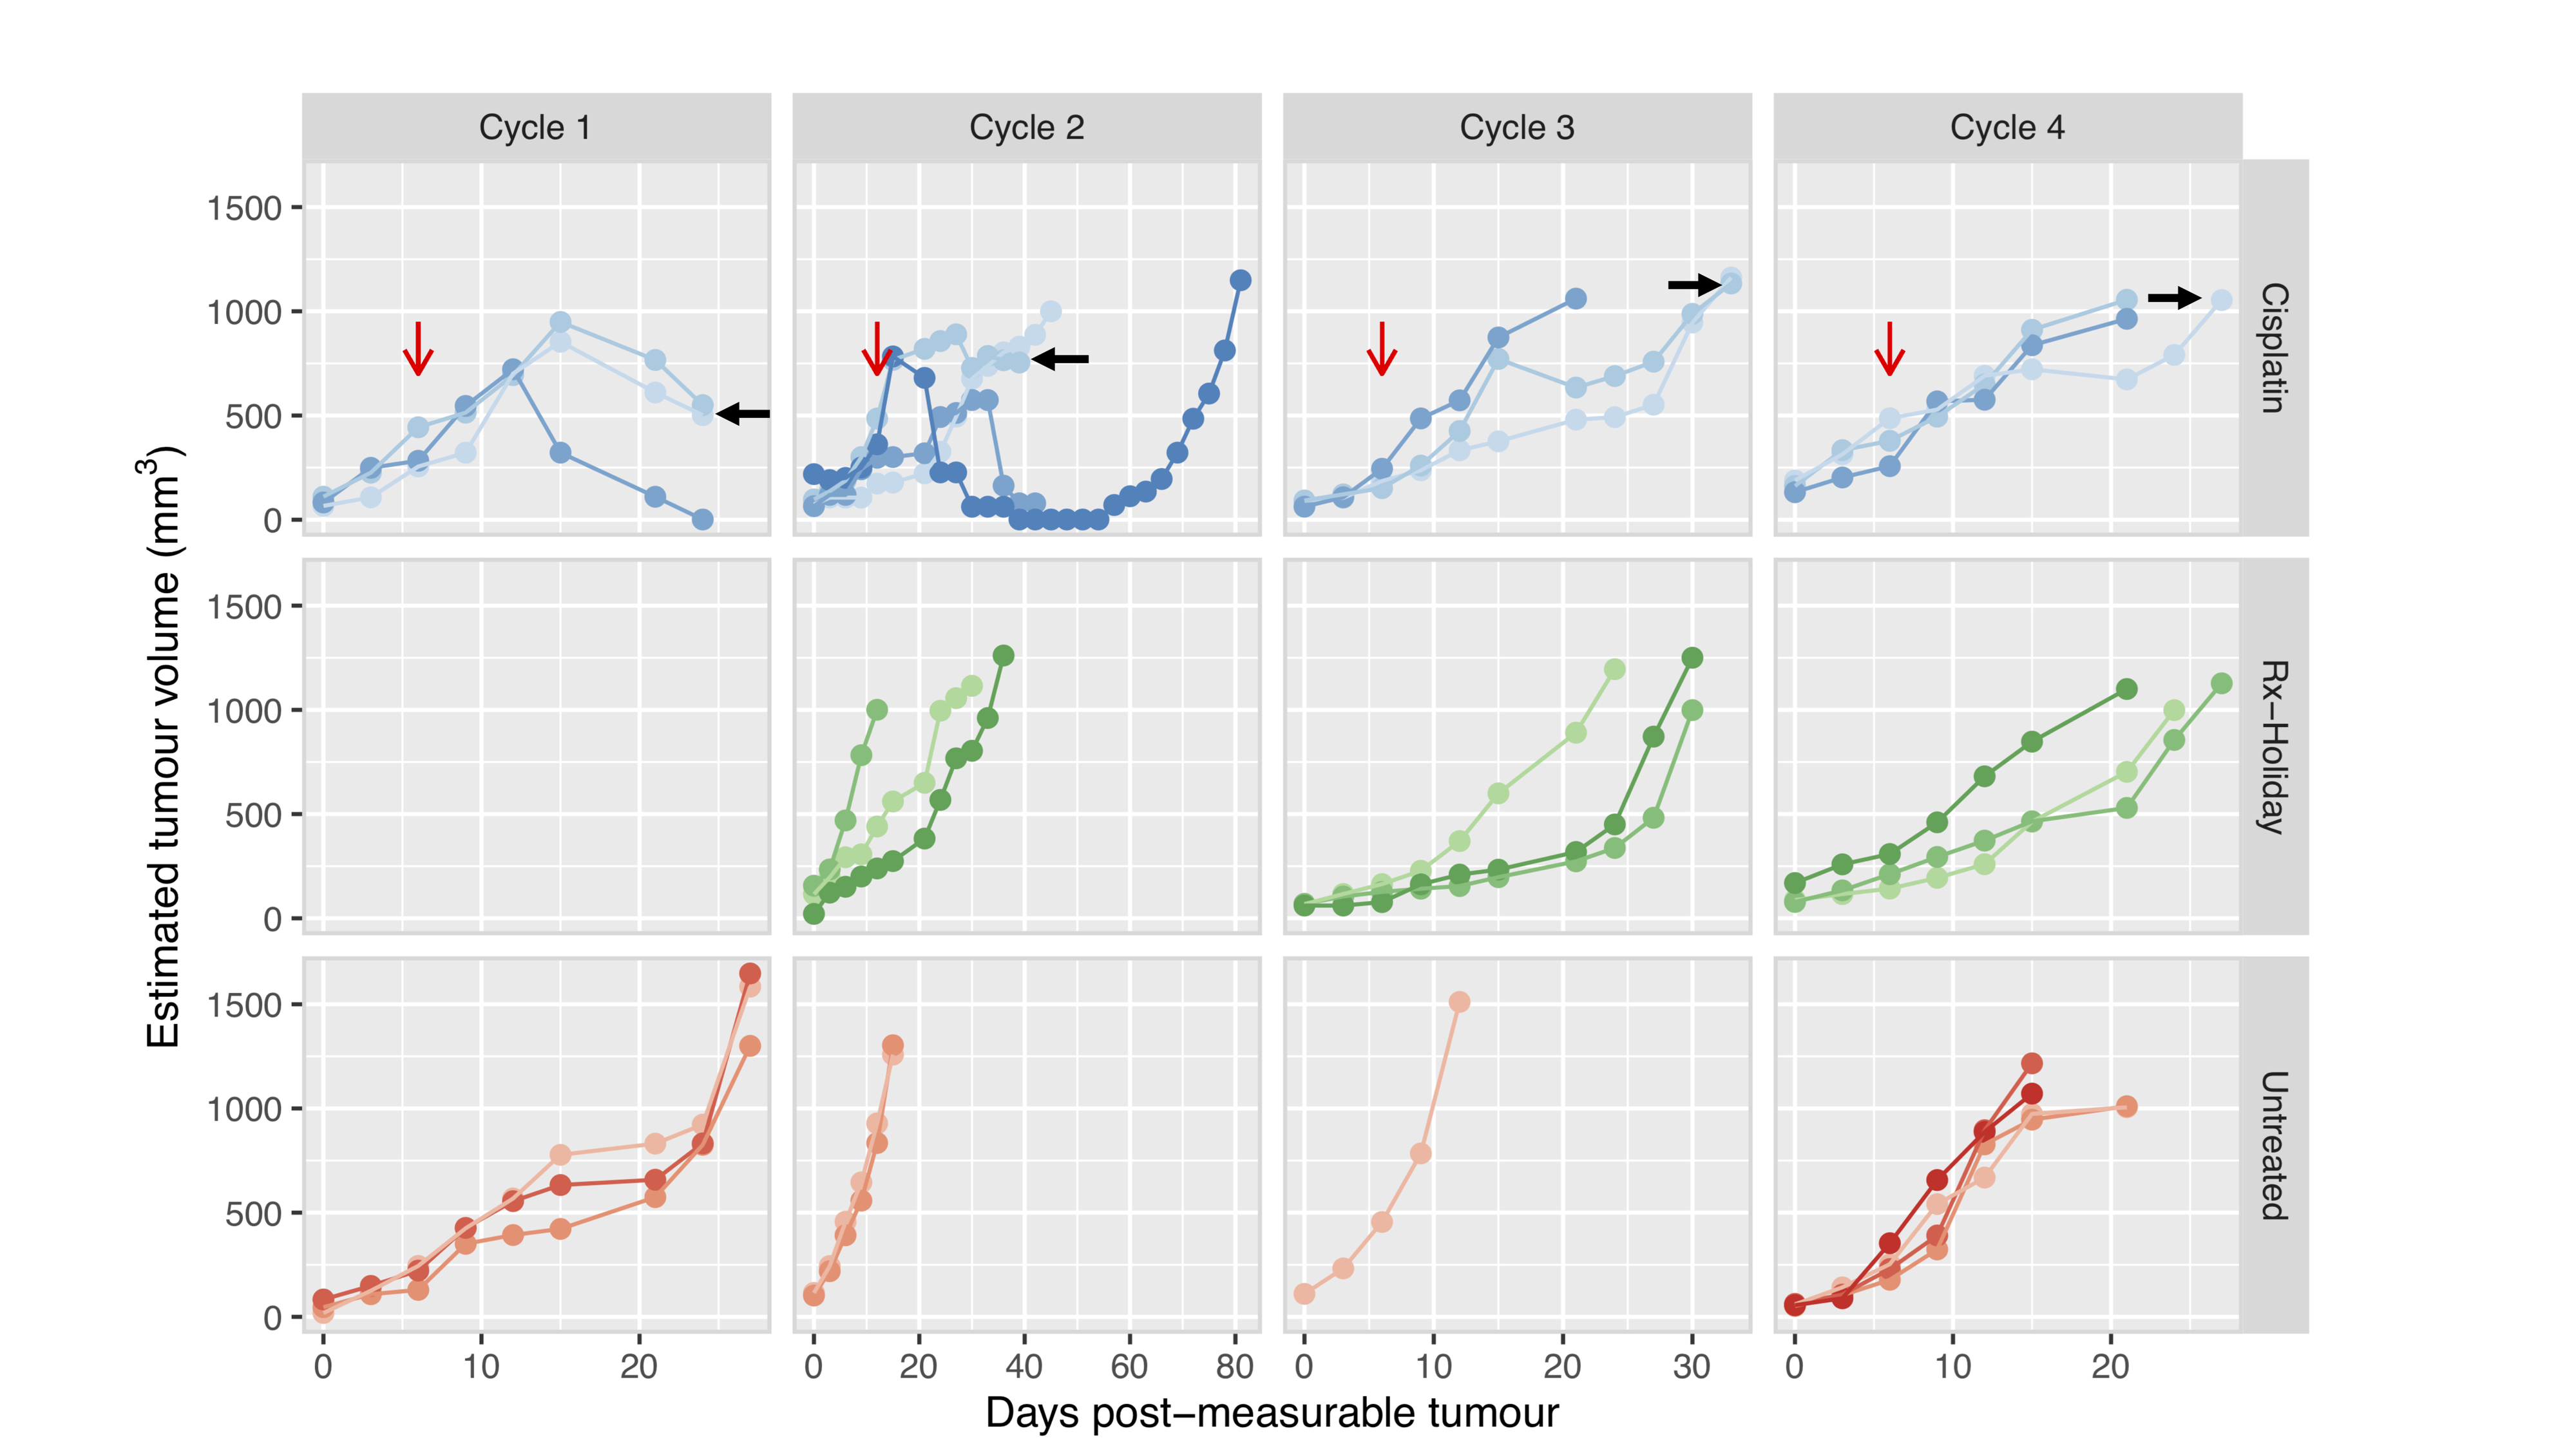
\includegraphics[width=\textwidth]{Figures/SA609allcyclescisplatin.pdf}
	
\caption[Representative growth curves from SA609 TNBC treated with cisplatin]
	{\small
	\textbf{Growth curves from SA609 TNBC treated with cisplatin.}
	   The vertical axis on the left side presents the tumor volume in cubic millimeters and on the right side presents the type of mice groups and their treatemnt status. Res arrows in the top panel indicates the time of start of drug treatment adn black arrow indicates the tumor that was taken to generate the next generation of mice.
	}
	\label{fig:Untreated timeseries growth curves only}
\end{figure}


%....................................................................


\begin{figure}
\centering
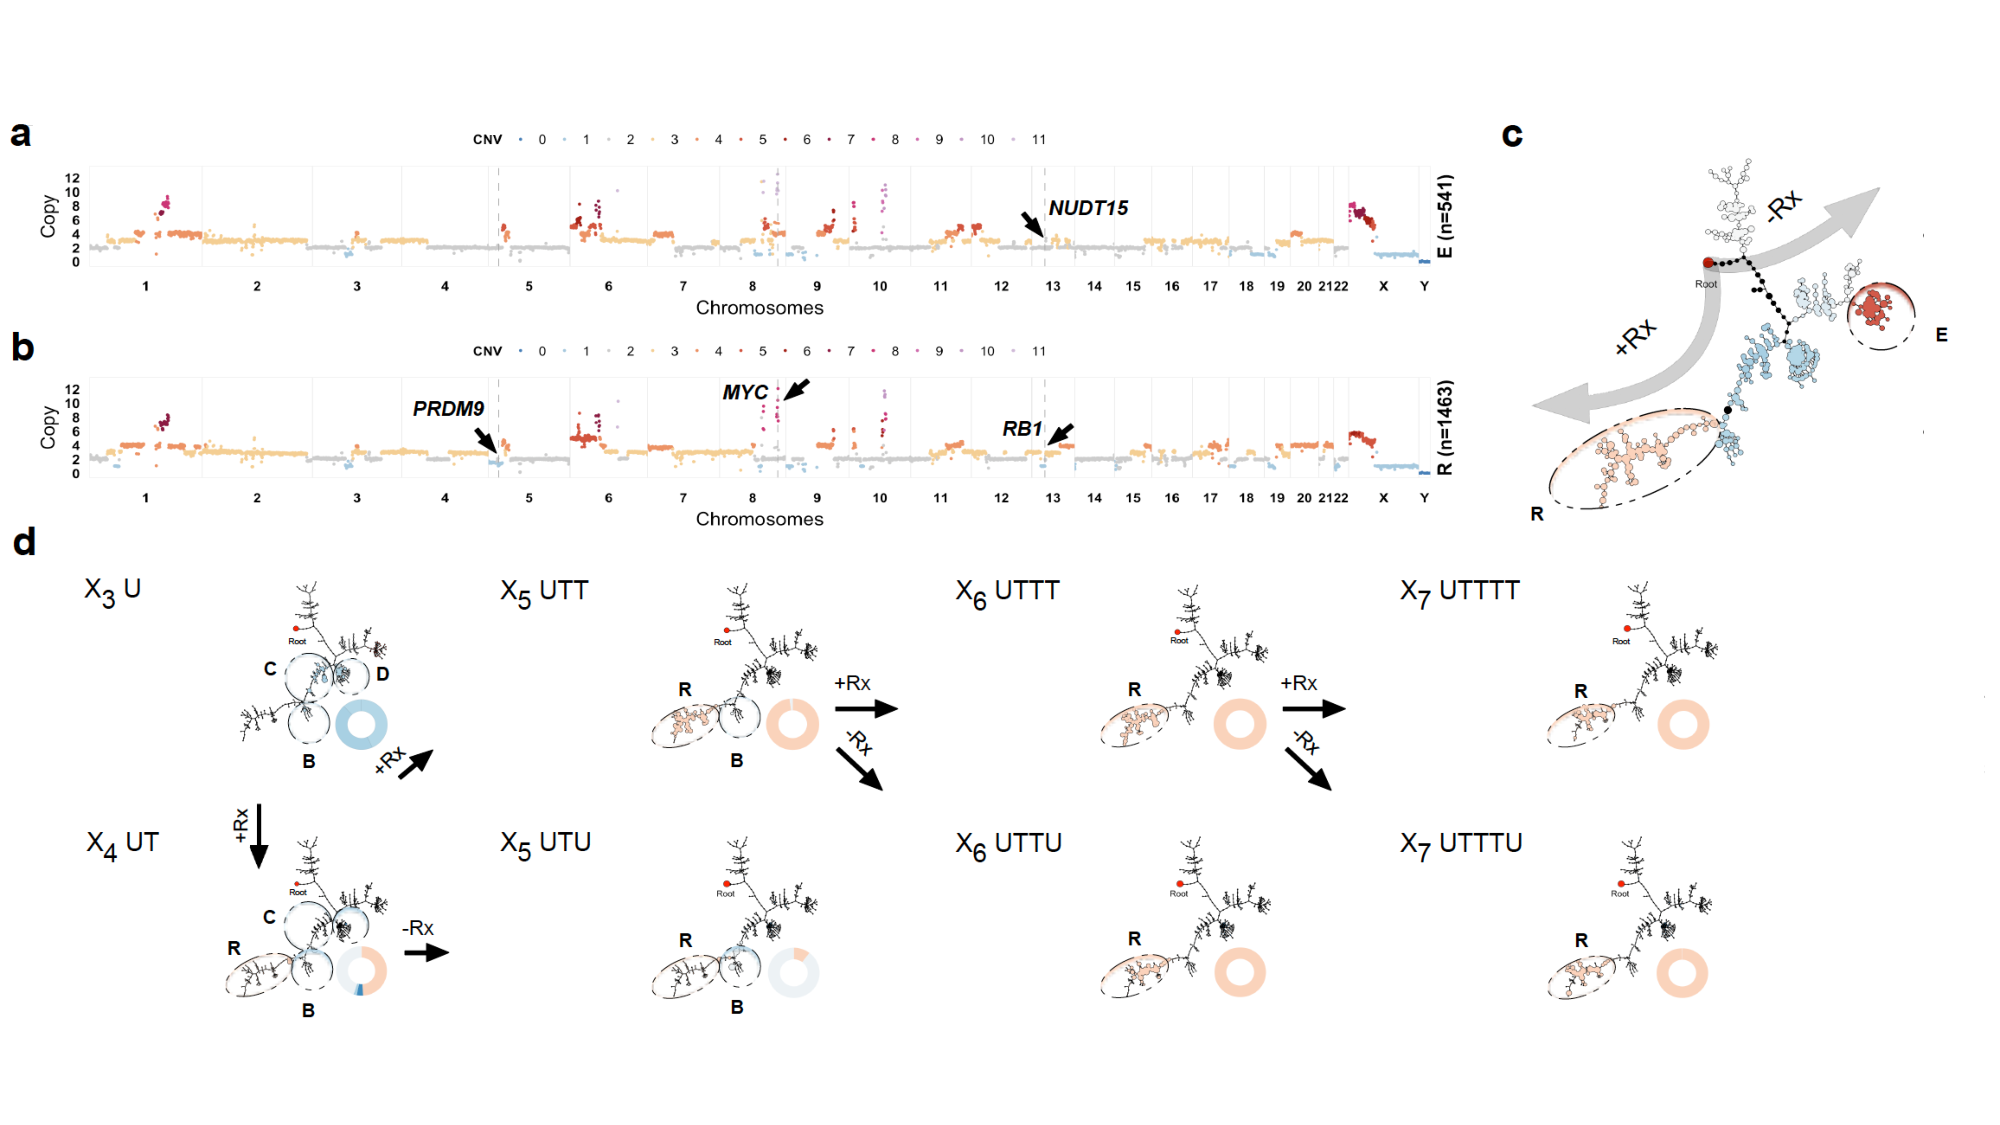
\includegraphics[width=\textwidth]{Figures/drugholidayfitnesscost.pdf}
	
\caption[Impact of cisplatin perturbation on fitness landscape in  SA609 TNBC PDX.]
	{\small
	\textbf{Impact of cisplatin perturbation on fitness landscape in  SA609 TNBC PDX.}
	  \textbf{(a)} Copy number genotype of clone E from untreated timeseries \textbf{(b)} Copy number genotype of clone R from treated timeseries (arrows indicate differences to clone E) \textbf{(c)} Clades with higher fitness in the untreated (-Rx) and treated (+Rx) series \textbf{(d)} Evolution as a function of drug treatment and drug holiday. Arrows indicate the path of serial passaging. For each sample, the phylogeny with clonal abundance from DLP+ is shown, reflecting selection..
	}
	\label{fig:Untreated timeseries growth curves only}
\end{figure}

%......................................................


\begin{figure}
\centering
\includegraphics[width=\textwidth]{Figures/SA609Rxnew.pdf}
	
\caption[SA609 TNBC PDX clonal dynamics with and without treatment.]
	{\small
	\textbf{SA609 TNBC PDX clonal dynamics with and without treatment.}
	    \textbf{(a)} Heatmap representation of copy number profiles of 841 cells, grouped in 6 phylogenetic clades 
	    \textbf{(b)} Phylogeny (simplified type II sitka tree) of cells over the SA609-Un-Rx where nodes are groups of cells (scaled in size by number) with shared copy number genotype and edges represent distinct genomic copy number change points (sitka markers). \textbf{(c)} Observed clonal abundances \textbf{(d)} distribution over magnitude of difference between selective coefficients of pairs of clones \textbf{(e, f, g, h)} Analogous plots for the treated branch (n=1,593 cells).
	}
	\label{fig:Untreated timeseries growth curves only}
\end{figure}

%.......................................................


\subsubsection {Clone-specifc cisplatin resistance has a fitness cost}
We next asked whether the clonal dynamics in the presence of cisplatin were reversible by exploring the drug holiday samples \textbf{(Figure 4.4 a, 4.6 d} \textit{X5 UTU}; \textit{X6 UTTU}; \textit{X7 UTTTU}). In the first drug holiday \textit{X5 UTU}, clonal composition reverted to consist predominantly of precursor clone B with 90\% abundance, and only 10\% abundance from clone R \textbf{(Figure 4.11}.  However, in \textit{X6 UTTU} and \textit{X7 UTTTU} no reversion was detected, and these populations consisted of  $>$99\% Clone R, similar to their on-treatment analogues. Thus, clonal competition in the absence of drug led to clones derived from the A-B clade out-competing clone R, and clone-specific cisplatin resistance thus has a fitness cost. Moreover, the genotype specificity of reversion between \textit{X4 UT} to \textit{X5 UTU} indicates that the clonal dynamics can be attributed to selection of genomically defined clones with differential fitness. 


\subsubsection{Fitness inversion is reproducible and not a stochastic effect}
Next, we examined whether the fitness inversion dynamics as a result of cisplatin chemotherapy in SA609 TNBC PDX model are due to stochastic effect or real.

We established parallel replicate timeseries of SA609 with cisplatin treatment shown as line 2 and line 3 in \textbf{figure 4.4 a}, and duplicate experiments of specific time points. We observed the same type of clonal dynamics as of line 1, briefly, a phylogenetic branch of the population which has low fitness in the untreated control branch is repeatedly observed to selectively expand on treatment. The precurosr clone B that gave rise to clone R in line 1, also gave rise to clone R1 in line 2 \textbf{(Figure 4.8 Line 2)}. Few time points analysis of line 3 also exhibited expansion of precursor clone B started giving rose to clone R, that was again found to be reversed in drug holiday sample of line 3 \textbf{(Figure 4.8 Line 3)}. This indicates that the fitness inversion is not a stochastic effect and establishes with precision that high fitness lineages in the untreated setting are selectively pruned, while low fitness lineages in the untreated setting selectively expand.
%.....................................................................

\begin{figure}
\centering
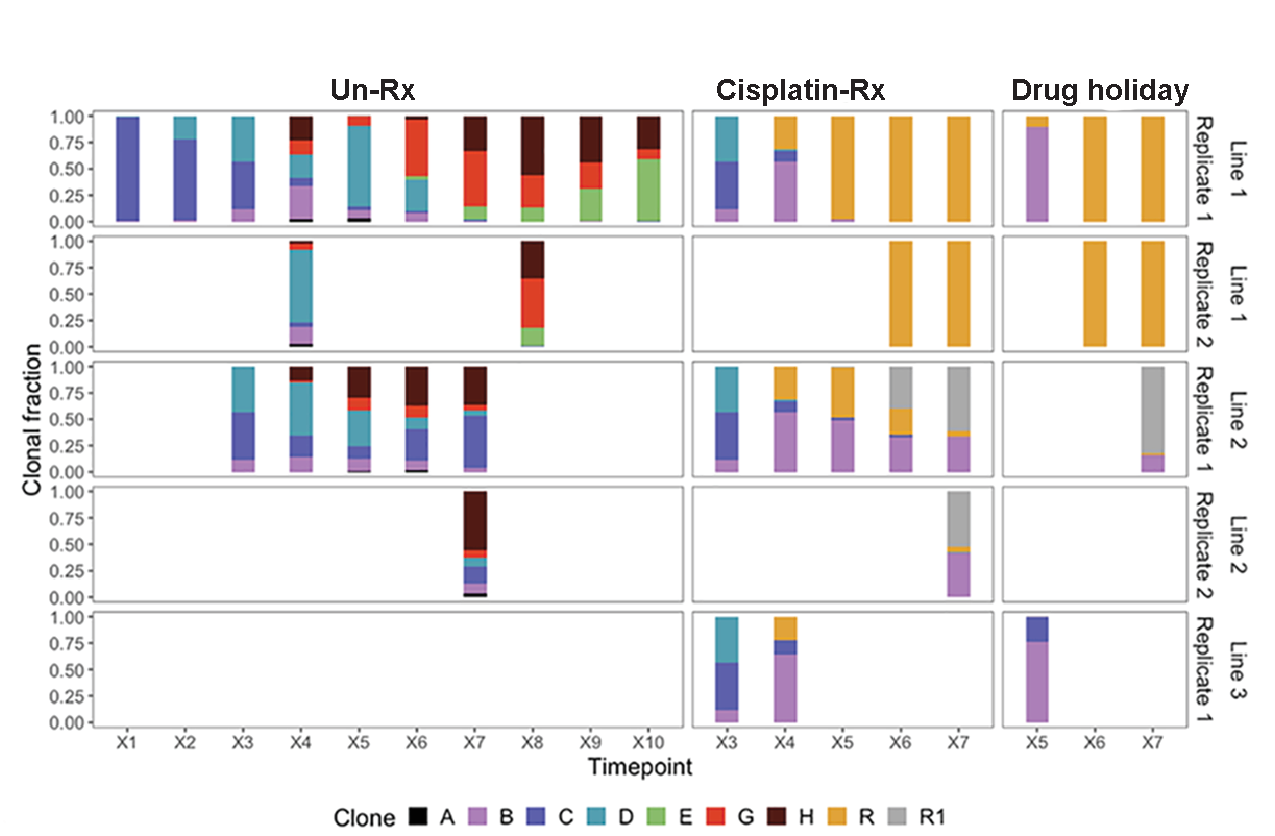
\includegraphics[width=\textwidth]{Figures/SA609barplotanalysis.pdf}
	
\caption[TNBC-SA609 PDX reproducible clonal dynamics with and without treatment]
	{\small
	\textbf{TNBC-SA609 PDX reproducible clonal dynamics with and without treatment.}
	    In both Line 1 and Line 2, the derivatives of clone B (R and R1) sweep the population. Line 3 confirms the same dynamics of clonal proportion with reversal of fitness at X5 in drug holiday sample where clone R is not fit in the absence of drug.
	}
	\label{fig:Untreated timeseries growth curves only}
\end{figure}

%.....................................................................

\subsection{Reversal of fitness landscape is generalizable under cisplatin selective pressure}
To test the generalizability of the observed drug selection dynamics with cisplatin, we performed the same experimental timeseries on two additional TNBC PDX models derived from new patients identified here as SA1035 and SA535 \textbf{(Figure 4.6 b,c)}. 

\subsubsection{Fitness inversion landscape also observed in SA1035-TNBC PDX with cisplatin}
Another independent PDX system with 14,170 single cells were generated where 4,444 passed the quality filters. The experimental design diagram is shown in \textbf{figure 4.4. b}.
Sc-WGS data collected from an untreated branch with five serial passages (X4, X5, X6, X7, and X8) \textbf{(Figure A.2 b)} with a total of 2,015 single cells. A parallel branch was treated with cisplatin starting at X5, X6, X7, and X8 comprising 1,596 filtered cells. 833 cells belonged to the drug-holiday timepoints \textbf{(Figure A.3 right top panel)}. Phylogenetic inference followed by cutting the tree yielded 11 clones \textbf{(Figure 4.9, 4.11)}. Clonal fractions over all timepoints in the untreated branch were A(0.097), B(0.140), C(0.087), D(0.160), E(0.266), F(0.010), G(0.058), H(0.053), I(0.065), J(0.018), and K(0.047). The abundance of clone A fell over time and it was chosen as the reference clone. Clone E rose from a clonal fraction of 0.028 at X4 to 0.69 at X8 and had the highest selection coefficient (1+s = 1.06 $\pm$ 0.0367). In the treated branch, clonal fractions were A(0.065), B(0.129), C(0.132), D(0.066), E(0.055), F(0.018), G(0.205), H(0.144), I(0.094), J(0.014), and K(0.078). In this regime, G (1+s = 1.01 $\pm$ 0.0123) and H (1+s = 1.02 $\pm$ 0.0135), which were among the clones with lower fitness in absence of treatment, rose to occupy 73\% at X8 while clone E (1 + s = 0.993 $\pm$ 0.0344) fell from about 10\% at X5 to undetectable at X8. Unlike SA609 TNBC, where we saw new clone emerging from existing precursor clone, a clone H with highest fitness coefficient in SA1035 TNBC was already present in the initial population at the start of drug treatment and exponentially increased with increasing drug cycles \textbf{(Figure\ref{4.9} c, g}. 

\subsubsection{High fitness clone emerged from the existing starting population with cisplatin in SA535-TNBC PDX}
 SA535 TNBC is a BRCA1 deficient patient derived tumour. We established a timeseries trransplants with treated and untreated branches similar to SA609 TNBC PDX \textbf{(Figure 4.6 b)}. 
 We generated a total of 15,302 single cells out of which 4,023 passed our quality filters.
 We acquired sc-WGS on 5 consecutively transplanted timepoints (X5, X6, X7, X8, X9) left untreated \textbf{(Figure A.2 b)} for a total of 1,341 single cells (mean = 335, $\sigma$ = 84.4 per timepoint). Simultaneously, we established a cisplatin treated timeseries starting from timepoint X6, and continued cisplatin treatment for 5 cycles up to X10, generating a total of 1,425 cells from scWGS (mean = 356, $\sigma$ = 159 per timepoint) from 4 cycles. A cut of the phylogenetic tree inferred over all cells in this series, resulted in 7 clones. In the untreated line, clonal fractions were A(0.003), B(0.702), C(0.034), D(0.006), E(0.006), F(0.013), and G(0.237).
Clone B was chosen as the reference clone as it had a monotonically decreasing clonal fraction trajectory in the untreated branch. Clonal trajectories were consistent with selection coefficients
with small relative differences in fitness \textbf{(Figure \ref{4.10}d)}. Clone G had the highest fitness (1 + s = 1.01 $\pm$ 0.00751) closely followed by clone C (1+s = 1.00 $\pm$ 0.0282) and the reference clone. In the treated branch, clonal fractions were A(0.156), B(0.066), C(0.140), D(0.194), E(0.182), F(0.151), and G(0.112). In this regime, clone A emerged with the highest selection coefficient (1 + s = 1.03
$\pm$  0.0152) followed by clone D (1 + s = 1.02 $\pm$ 0.0116). Notably clones A and D had low fitness values under no treatment, whereas clones G (1+s = 1.01 $\pm$ 0.0115) and C (1+s = 1.02 $\pm$ 0.0119) had low fitness coefficients under treatment. Like SA1035 clonal dynamics, SA535 also displayed high fitness clone H emerging from already present initial population,  taking survival advantage under drug selection.

%.................................................................


\begin{figure}
\centering
\includegraphics[width=\textwidth]{Figures/SA1035Rxnew.png}
	
\caption[SA1035 TNBC PDX timeseries clonal dynamics under drug perturbation]
	{\small
	\textbf{SA1035 TNBC PDX timeseries clonal dynamics under drug perturbation.}
	    \textbf{(a)} Heatmap representation of copy number proles of
2,015 cells, grouped in 11 phylogenetic clades  \textbf{(b)}Phylogeny (simplified type II sitka tree) of cells over the SA1035-Un-Rx where nodes are groups of cells (scaled in size by number) with shared copy number genotype and edges represent distinct genomic copy number change points (sitka markers). \textbf{(c)} Observed clonal abundances \textbf{(d)} distribution over magnitude of difference between selective coefficients of pairs of clones \textbf{(e, f, g, h)} Analogous plots for the treated branch (n=1,596 cells).
	}
	\label{fig:SA1035Rxnew}
\end{figure}


%.....................................................................

\begin{figure}
\centering
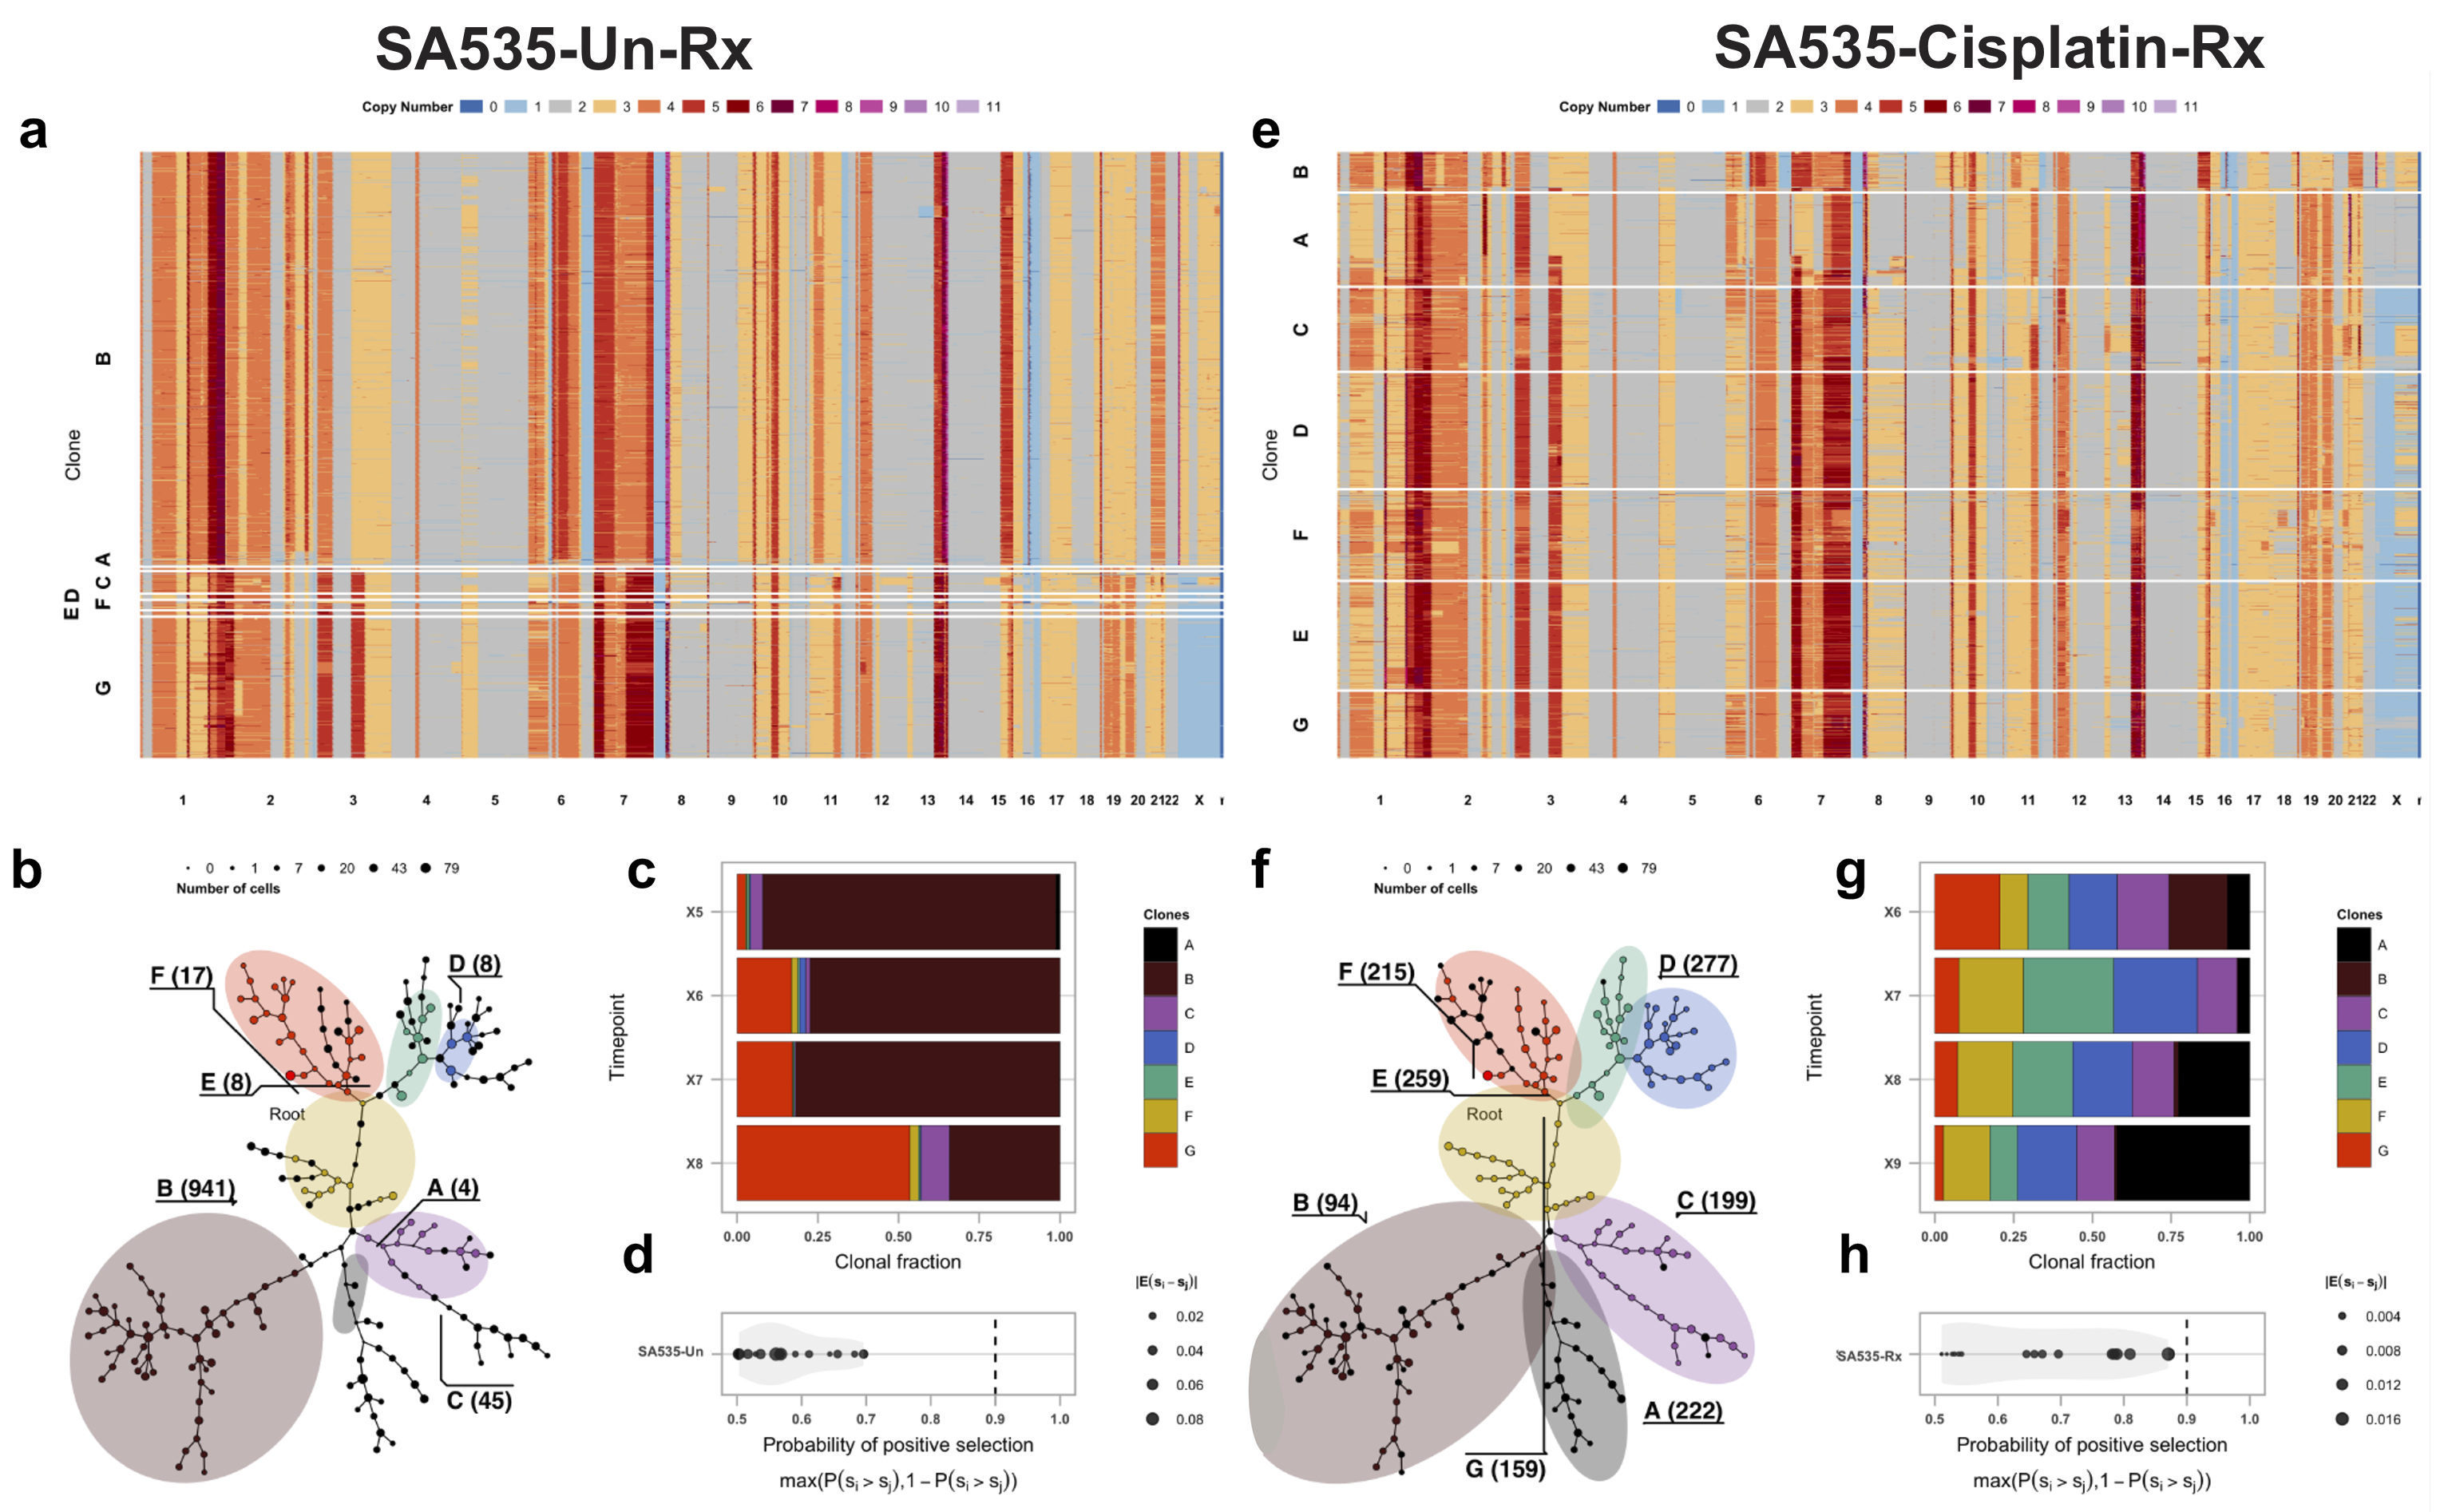
\includegraphics[width=\textwidth]{Figures/SA535analysis.pdf}
	
\caption[SA535 TNBC PDX timeseries clonal dynamics under drug perturbations]
	{\small
	\textbf{SA535 TNBC PDX timeseries clonal dynamics under drug perturbations.}
	     \textbf{(a)} Heatmap representation of copy number profiles of
2,015 cells, grouped in 11 phylogenetic clades  \textbf{(b)}Phylogeny (simplified type II sitka tree) of cells over the SA535-Un-Rx where nodes are groups of cells (scaled in size by number) with shared copy number genotype and edges represent distinct genomic copy number change points (sitka markers). \textbf{(c)} Observed clonal abundances \textbf{(d)} distribution over magnitude of difference between selective coefficients of pairs of clones \textbf{(e, f, g, h)} Analogous plots for the treated branch (n=1,425 cells).
	}
	\label{fig:SA535analysis}
\end{figure}

%...............................................................

\begin{figure}
\centering
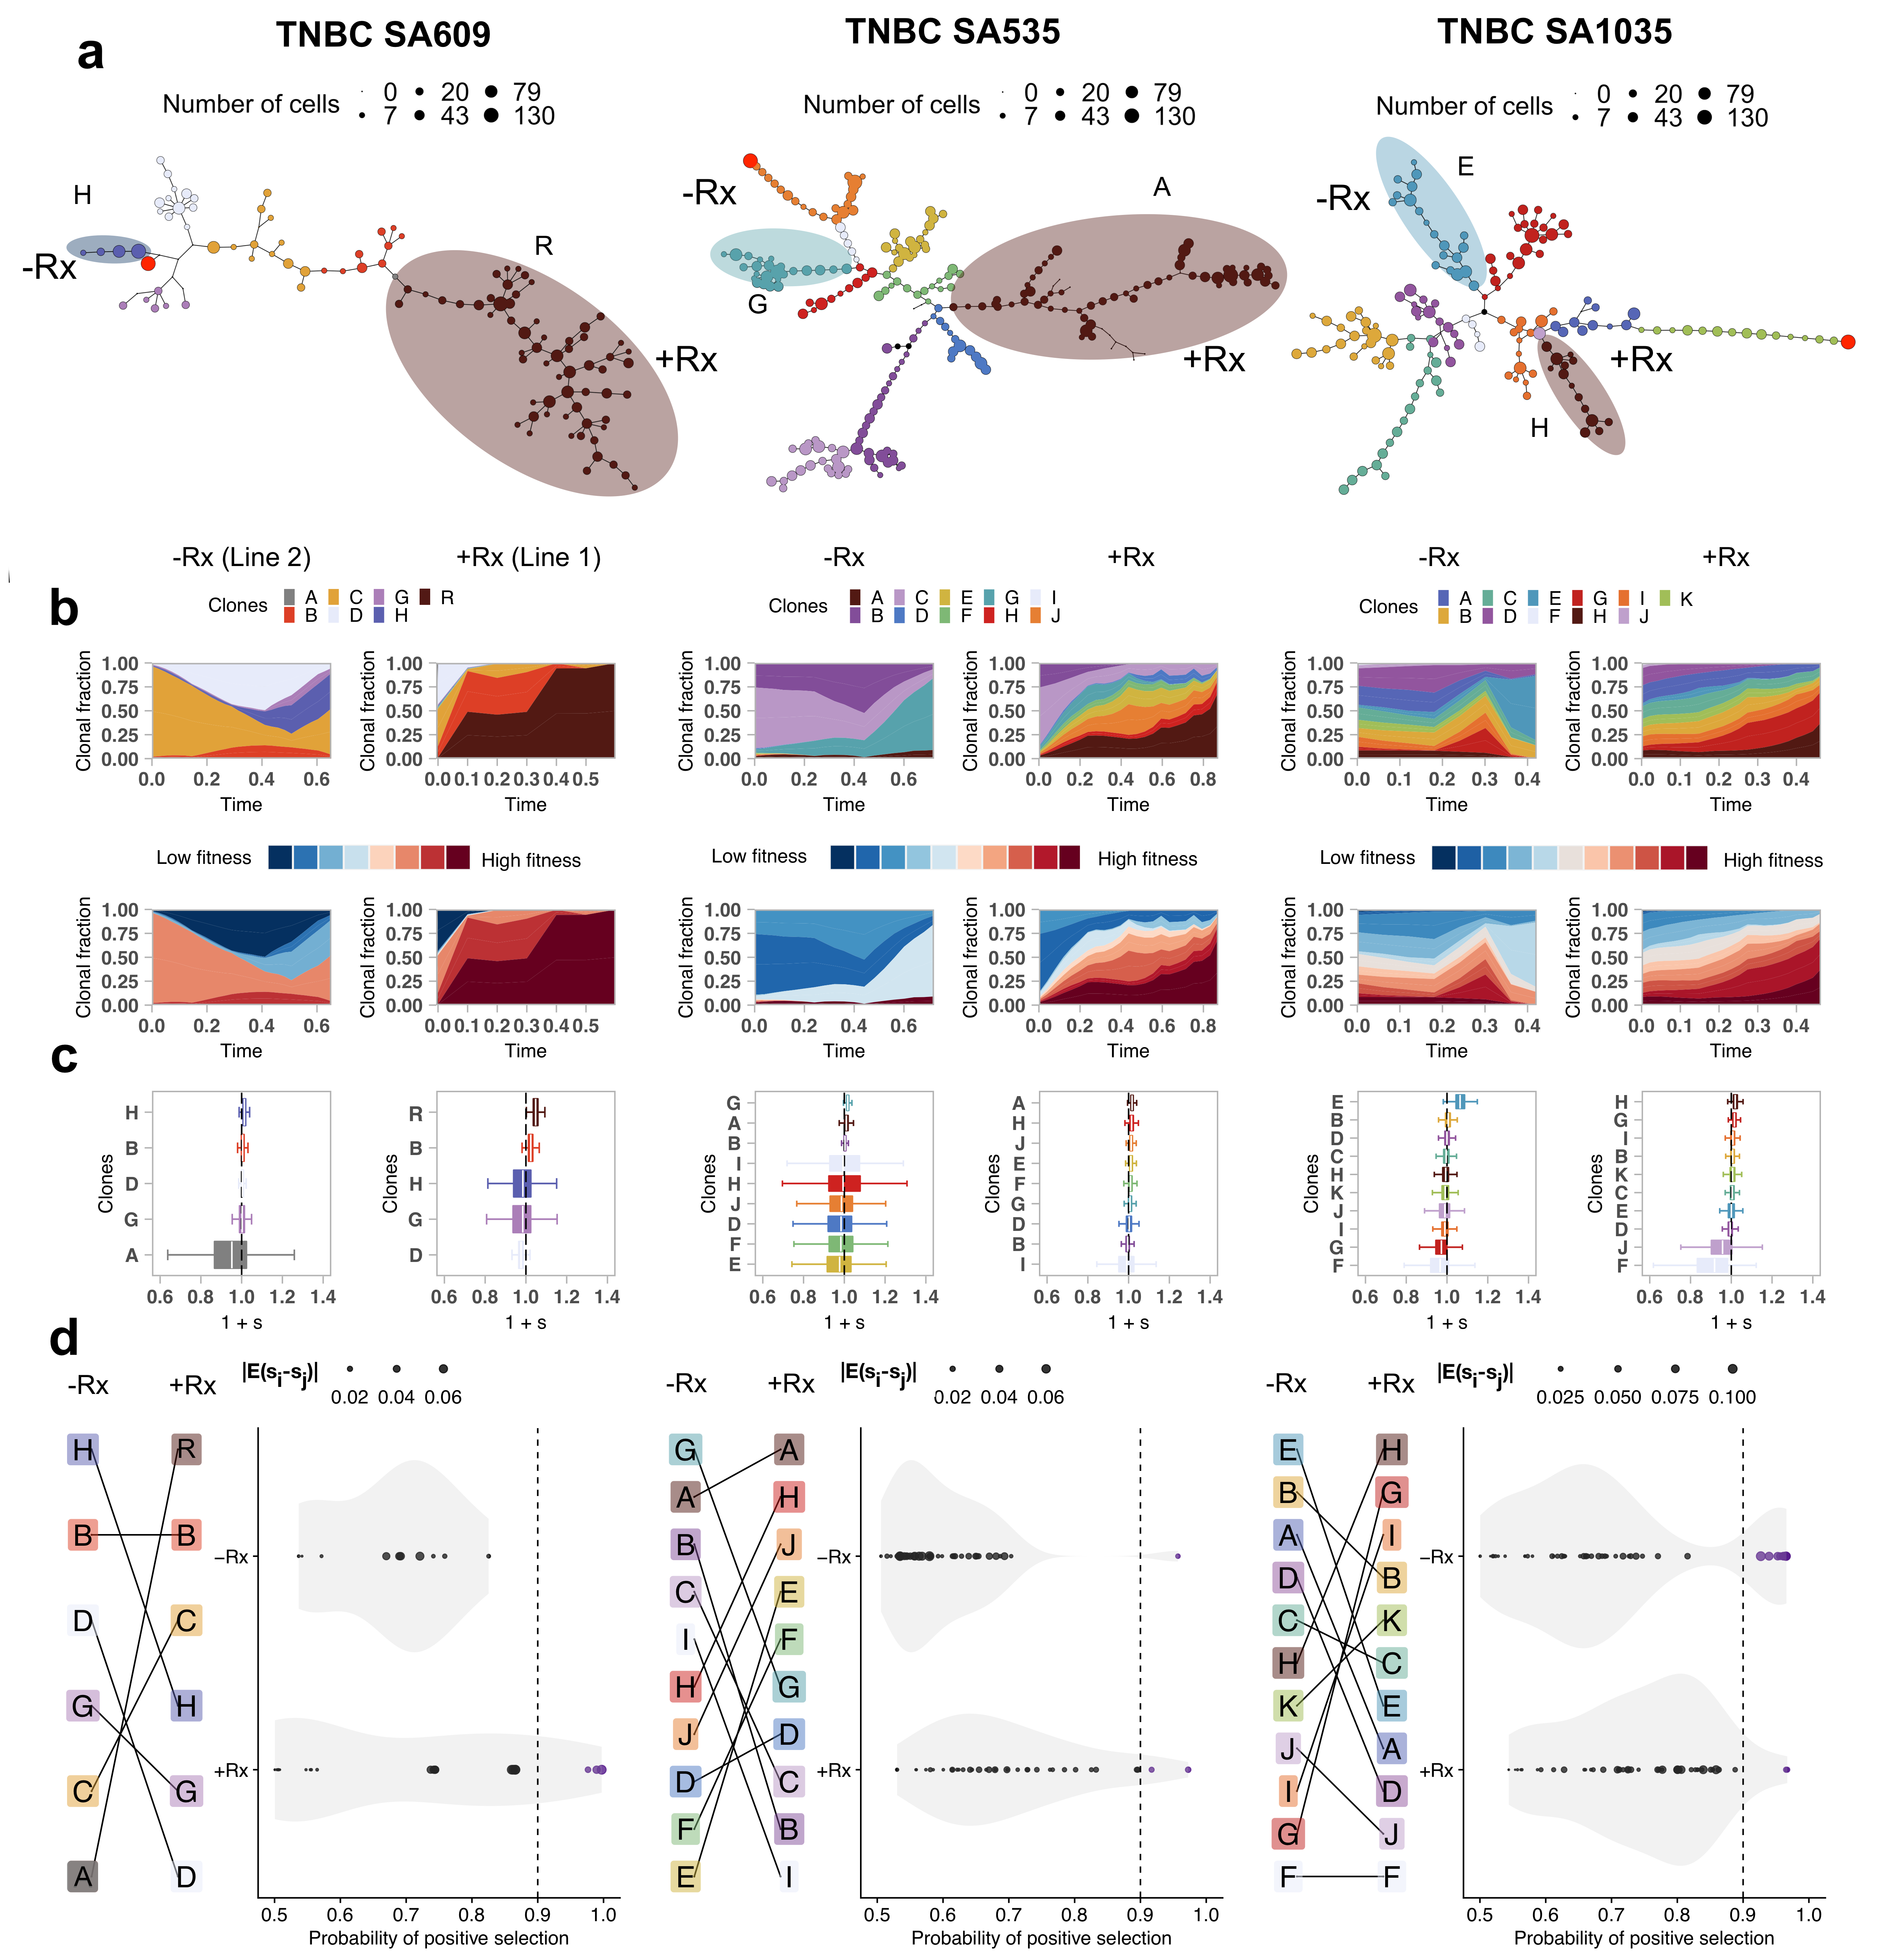
\includegraphics[width=\textwidth]{Figures/landscapefitness.pdf}
	
\caption[Fitness landscape reversal in early cisplatin treatment in TNBC PDX models.]
	{\small
	\textbf{TNBC PDX models exhibiting fitness landscape inversion in early cisplatin treatment.}
	     We observe in 3 independent TNBC PDX lines that clone specific resistance to cisplatin treatment arises. In all three cases, clones with low fitness under no treatment exhibit high fitness under the treatment regime. In each panel, the left and right sub-panels are from the untreated and treated branches respectively \textbf{(top)} Phylogenetic trees showing clones sorted by their median selection coefficient in -Rx and +Rx regimes  \textbf{(middle)} inferred trajectories, and  \textbf{(bottom)} selection coefficients of \texttt{fitClone} model fits to each branch.
	}
	\label{fig:landscapefitness}
\end{figure}
%.....................................................................


\subsubsection{Fitness inversion summary from TNBC under cisplatin regime }
In the TNBC-SA609 system the fitness landscape is inverted wherein
clones more fit in the untreated regime (H, D) are less fit in the treated regime, whereas less fit clones in the untreated regime (A, B) are the most fit clones under treatment. This pattern is
mirrored in two independent TNBC PDX lines treated with cisplatin, namely TNBC-SA535 and TNBC-SA1035. In TNBC-SA535, clones G, C, and B are drug-sensitive, meaning they could not survive drug pressure, while A and D are drug resistant because they are showing high fitness coefficient in the presence of drug. Also,the former have higher relative fitness in untreated versus treated regimes, while the latter exhibit an inverted fitness pattern. Similarly, in TNBC-SA1035, drug-sensitive clones consist of clones E, B, and A, while the drug-resistant group comprises clones H, I, and G. From untreated
to treated, the first group goes from high to low fitness, while the second group goes from low to high fitness. \textbf{Figure 4.11} summarises the reversal in the fitness landscape in response to cisplatin treatment in TNBC-PDX model systems.

%...........................................................


\subsection{Comparison of fitness landscape of platinum and CX-5461 in TNBC PDX timeseries}
So far we have applied only platinum compound to TNBC PDX in a time series manner to track copy number based genomic clones. Now we investigate whether establishing the same patients tumor model of forced amplified evolution, with another drug, CX-5461, could help to interpret the clonal relationship and their fitness within the same tumor type.
One TNBC SA535, was BRCA1 deficient (HRD-Dup), so we developed a repeated CX-5461 drug exposure timeseries model same experimental design \textbf{(Figure 2.2 a)} to compare cisplatin induced clonal dynamics. Platinum (cisplatin) is a standard chemotherapeutic agent whereas, CX-5461 is a G4 quadruplex stabilizer drug, known to have synthetic lethality with BRCA deficiency.

% waiting for correct data from Hoa: We established a timeseries SA535 TNBC PDX with treated and untreated branches similar and in parallel to cisplatin \textbf{(Figure 4.12 a)}. We collected sc-WGS from consecutively transplanted untreated timepoints (X4, X5, X6, X7, X8, X9) for a total of 1,341 single cells (mean = 335, $\sigma$ = 84.4 per timepoint). Simultaneously, we established a cisplatin treated timeseries starting from timepoint X6 to X10, CX-5461 treated timeseries in parallel and continued CX-5461 treatment for 5 cycles from X5 to x9 to X10, generating a total of 1,425 cells from sc-WGS (mean = 356, $\sigma$= 159 per timepoint).

Tumor growth curves displayed progressively less response of the tumors in last cycle of drug as comnpared to the first, indicating initiation of drug resistance to both cisplatin and cX-5461 \textbf{Figure 4.12 b, c}. Positive growth kinetics started earlier in cisplatin tumors as compared to CX-5461.
%......................................................

\begin{figure}
\centering
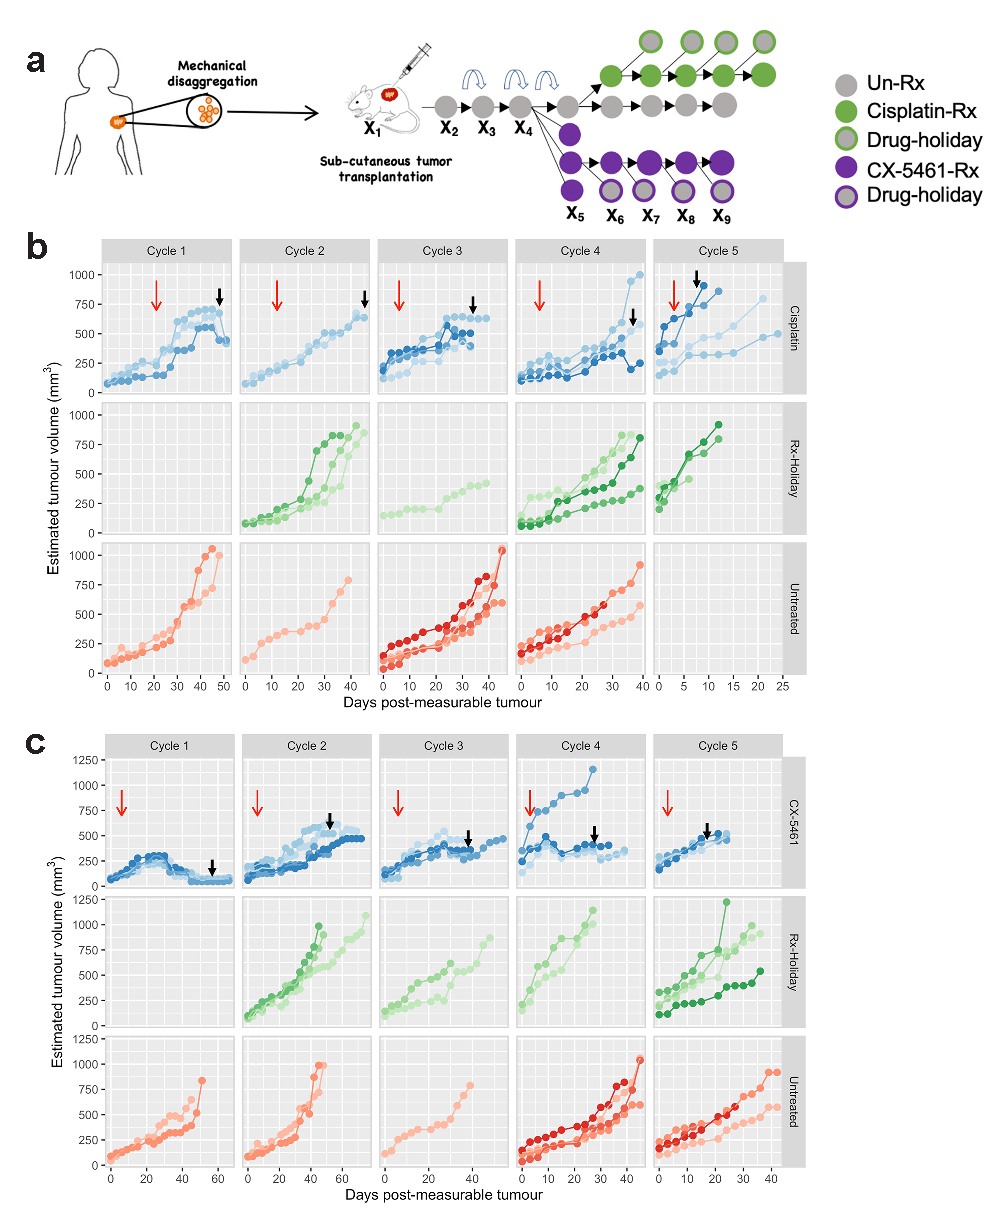
\includegraphics[width=\textwidth]{Figures/SA535CX5461.pdf}
	
\caption[SA535 TNBC PDX timeseries with cisplatin and CX-5461]
	{\small
 \textbf{SA535 TNBC PDX timeseries with cisplatin and CX-5461.}
	    	Vertical axis on right indicates the tumor status. The top bar gives cycle numbers and left vertical axis gives tumor measurements. Horizontal axis are days post measurable tumors\textbf{(a)} Experimental overview and passaging details of start and end of cisplatin and CX-5461 treatments. Red arrows point to the start of treatemnt and black arrows point to the tumor rdigested for sc-WGS.
	   \textbf{(b)} Growth curves of cisplatin treated tumors
	    \textbf{(c)} Growth curves of CX-5461 treated tumors.
	}
	\label{fig:SA535CX5461}
\end{figure}

%......................................................................



\begin{figure}
\centering
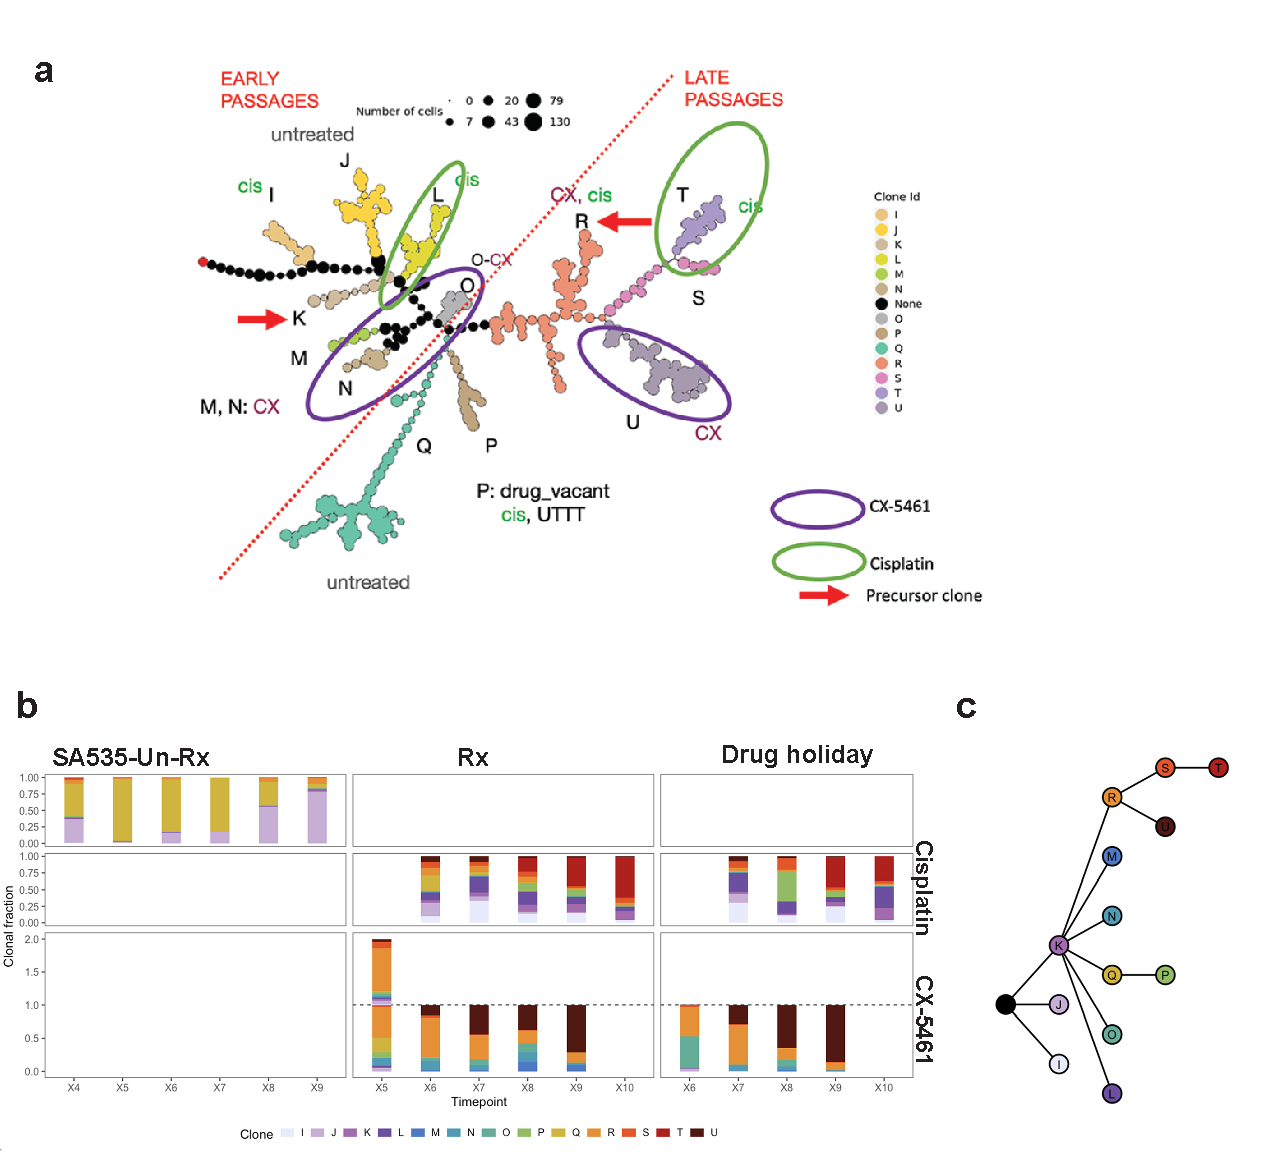
\includegraphics[width=\textwidth]{Figures/SA535-family_FK.pdf}
	
\caption[Combined data analysis of SA535 with cisplatin and CX-5461]
	{\small
	\textbf{Combined data analysis of SA535 with cisplatin and CX-5461.}
	    \textbf{(a)} Combined computed phylogenetic tree indicating purple circled clnes from CX-5461 and green from cisplatin treated. Red dotted arbitrary line separating the early and late time points dynamics of clones. 
	    \textbf{(b)} Bar plots showing clonal composition at each time point. Vertical axis shows the clonal frraction   and horizontal axis presents the passage timepoint.
	     \textbf{(c)} Simplified way to present clonal lineage tree matching the bars composition in \textbf{(b)}.
	}
	\label{fig:SA535-family_FK}
\end{figure}

%...............................................................

\subsubsection{Drug resistant clones arise from the same precursors}
that the resistant branches S and T for cisplatin and U for CX-5461, both derive from clone R, which is present early in variable proportions early in the two branches, but does not have fitness in the untreated, present but at a very minor proportion. So independently, drug resistance has apparently a favored clonal starting point in this PDX. I think this is a striking result. It will be interesting learn what is different about R compared with Q, K, J etc. 








\section{Discussion}
SA609 TNBC drug holiday data suggest the impact of cisplatin selective pressure on the starting tumour cell population is reversible while genomic clonal competition with precursor clones is still possible, but dominates the population once the evolutionary bottleneck narrows and purifes the population.

The fitness landscapes are inverted as a result of cisplatin chemotherapy in a triple negative breast cancer PDX model.  We have generated replicate observations in PDX models in two ways: parallel replicate timeseries transplants (Figure 3) with cisplatin treatment, and duplicate experiments of specific time points (Figure 4). In untreated timeseries (Fig 4 left panel), we observe repeated expansion of clone H, relative to lower fitness clones (e.g. clone D). Furthermore, in treated series, we observe the same clonal dynamics - namely that a phylogenetic branch of the population which has low fitness in the untreated control branch is repeatedly observed to selectively expand on treatment.  Notably, we remark in triplicate lines,  highly congruent dynamics with the introduction of treatment between X3 and X4.  Furthermore within lines, we observe through duplicate samplings that the clonal expansion patterns are repeatedly observed. With these repeat experiments, we note that the starting population structure is not deterministic of clonal abundance of future population structure.  We attest that while stochastic effects of sampling cannot be ruled out, the monotonic trajectories of clones and repeated observations strongly suggest variation in fitness as a primary determinant. In additional series added to this revision (Fig 3, 5, 6) we note that the starting point of treatment experiments harbours a more balanced representation of high and low fitness clones, and therefore are less subject to the sampling bias raised by the reviewer.  In these 2 series, similar inversions of the fitness landscape are observed.  Together, the replicate experiments and addition of 2 new TNBC PDX series indicate that the fitness inversion is not a stochastic effect and establishes with precision that high fitness lineages in the untreated setting are selectively pruned, while low fitness lineages in the untreated setting selectively expand. The observation that drug resistance can have a fitness cost also points to an underlying mechanism of retained sensitivity in early treatment.




